\newcommand{\Approx}[0]{\textsc{NearDup}}
\newcommand{\Exact}[0]{\textsc{ExactSubstr}}
\newcommand{\Original}[0]{\textsc{Original}}
\sethlcolor{lightyellow}
\newcommand{\pl}[1]{\hl{#1}}

\definecolor{pink}{RGB}{255, 71, 76}
\definecolor{kelleygreen}{RGB}{0, 147, 55}
\definecolor{purple}{RGB}{102, 102, 225}
\definecolor{lightyellow}{RGB}{255, 252, 187}

\chapter{Memorization}
\label{chap:memorization}

\section{Motivation}
Machine-generated text is most undetectable when it looks exactly like its training data.
In fact, the log-likelihood loss used during training explicitly encourages models to be able to exactly reproduce their training data.
The result is models that are capable of exactly reproducing multi-paragraph sequences verbatim from their training data.
As models have grown from millions to trillions of parameters \citep{fedus2021switch}, with their training sets similarly growing from millions to trillions of tokens, they  are at increased risk of memorizing their training data.
The problem is made worse by the fact that these enormous datasets are only minimally curated.
For example, Carlini et al. \citep{carlini2020extracting} found that while most instances of memorization are innocuous, such as news articles or religious text, models are also capable of memorizing things like contact information or the names of real individuals (referenced outside of news contexts).
This sort of memorization is harmful if it breaches expectations of privacy or content ownership from those whose data is included in the train set.
Memorizaiton also reduces generalizability if models are biased toward examples that are not representative of the underlying distribution of natural language.

In this chapter, we quantify the properties which raise the risk of memorization, notably the size of the model and the number of times a document occured during training.
We also show how passing in a long prompt to the model increases the chance we will extract memorized content.
Finally, we describe one actionable step--thorough dataset deduplication--which can be employed before training to diminish the risk of memorization.


\section{Quantifying the Factors that Influence Memorization}
\label{section:quantifying_memorization}

\subsection{Introduction}

It is important to  quantify factors that lead to increased memorization of a model's training set.
% understand to what extent these future models may \emph{memorize} their training data.
%
Indeed, recent work has shown that \emph{training data extraction attacks} are a practical threat for current language models ~\citep{carlini2020extracting};
an adversary interacting with a pretrained model can extract individual
sequences that were used to train the model.

While current attacks are effective, they only represent a lower bound on how much memorization occurs in existing models.
%
For example, by querying
the GPT-2 language model, \citet{carlini2020extracting} (manually) identified just $600$ memorized training examples out of a $40$GB training dataset.
%
This attack establishes a (loose) lower bound that at least
0.00000015\%
% $1.5\times10^{-7}\%$
of the dataset is memorized. % The authors hypothesized that this lower bound is likely very loose.
%However, in our experiments, we find \todo{memorization}
% 
In contrast, we are able to show that the 6 billion parameter 
GPT-J model \citep{gpt-neo,gpt-j} memorized at least $1\%$ of its training dataset: The Pile (\cite{gao2020pile}).

In addition to these loose estimates of models' memorization capabilities, there is a limited understanding of how memorization varies across different neural language models and datasets of different scales.
%
Prior studies of memorization in language models either focus on models or datasets of a fixed size~\citep{carlini2019secret, zhang2021counterfactual, thakkar2020understanding} or identify a narrow memorization-versus-scale relationship~\citep{carlini2020extracting, lee2021deduplicating}.
\citet{mccoy2021raven} broadly study the extent to which language models memorize, but their focus is on how to avoid the problem and ensure novelty of model outputs, rather than on studying model risk through identifying maximum memorization.
%how to maximize memorization to study model risk.

The research presented in this section addresses both of the above open questions by 
comprehensively quantifying memorization across three families of neural language models and their associated datasets.
%
We leverage access to each model's original training set to provide order-of-magnitude more precise bounds on the amount of extractable data than in prior works.

To construct a set of prompts from the model's training set, 
we feed varying-length prefixes of the training data back into the trained model, and verify whether the model has the ability to complete the rest of the example verbatim.

%
This allows us to measure memorization across models, datasets, and prompts of varying sizes. We identify three properties that significantly impact memorization:

\begin{enumerate}
    \item \textbf{Model scale:} %doubling the number of parameters in a model increases memorization by a factor of TODO.
    Within a model family, larger models memorize $2$-$5\times$ more data than smaller models. 

    \item \textbf{Data duplication:} Examples repeated more often are more likely to be extractable.
    
    \item \textbf{Context:} It is orders of magnitude easier to extract sequences when given a longer surrounding context.
\end{enumerate}

Our analysis suggests that future research on neural language modeling will need to take steps
to prevent future (larger) models from memorizing their training datasets.


\subsection{Related Work}

There is extensive prior work that qualitatively studies memorization in neural language models. Even constrained to just \emph{extraction}, prior work has demonstrated that it possible to recover various forms of memorized data including URLs, phone numbers, or other forms of personal information~\citep{carlini2020extracting, ziegler2021copilot}, or in other work, synthetically injected ``canaries''~\citep{carlini2019secret, henderson2017ethical, thakkar2020understanding, thomas2020investigating}.
%
However most of these works are qualitative and aim to demonstrate the existence of extractable data, rather than precisely quantifying how much models memorize.
For example, the unprompted memorization evaluation of \citet{carlini2020extracting} found just 600 examples of memorization in GPT-2.
%
Our paper aims to establish much tighter approximations to the fraction of a dataset that can be adversarially extracted.

Our analysis is relevant to the broad literature on privacy attacks on machine learning.
For example, membership inference attacks~\citep{shokri2017membership, yeom2018privacy} allow an adversary to detect the presence of a given example in a model's training dataset, and other forms of data leakage permit an adversary to learn dataset properties \citep{ganju2018property,fredrikson2015model}.
We focus on extraction attacks due to their relevance for language modeling---extraction demonstrates significant leakage from a model, and grows with data duplication \citep{lee2021deduplicating}, a common feature of large-scale text datasets.

%TODO
%\cite{} show that the performance of code understanding models suffers when training sets have duplicates.

Various formulations of memorization in deep neural networks have been studied in previous papers~\citep{carlini2019secret,carlini2020extracting,feldman2020neural,zhang2021counterfactual,colinpaper}. A detailed comparison with those existing formulations is presented in Section~\ref{sec:mem-def}.
% Along this line, \citet{zhang2021counterfactual} formulated a notion of counterfactual memorization to characterize memorized training examples that are not duplicated. Our observation of the impact of duplication on memorization is consistent with theirs, and we provided a quantitative study to precisely characterize it.
One leading general memorization definition is differential privacy~\citep{dwork2006calibrating}, which is formulated around the idea that removing any user's data from the training set should not change the trained model significantly.
However, while differential privacy protects a single user's private information, it is ineffective for memorization of duplicated data and does not capture the complexity of linguistic data~\citep{brown2022does}.
Also, differentially private deep learning algorithms~\citep{abadi2016deep} generally suffer from expensive computation, slow convergence, and poor model utility, despite recent advances~\citep{anil2021large}.


\begin{figure*}
\hspace{-2em}
    \centering
    \begin{subfigure}[b]{0.27\textwidth}
        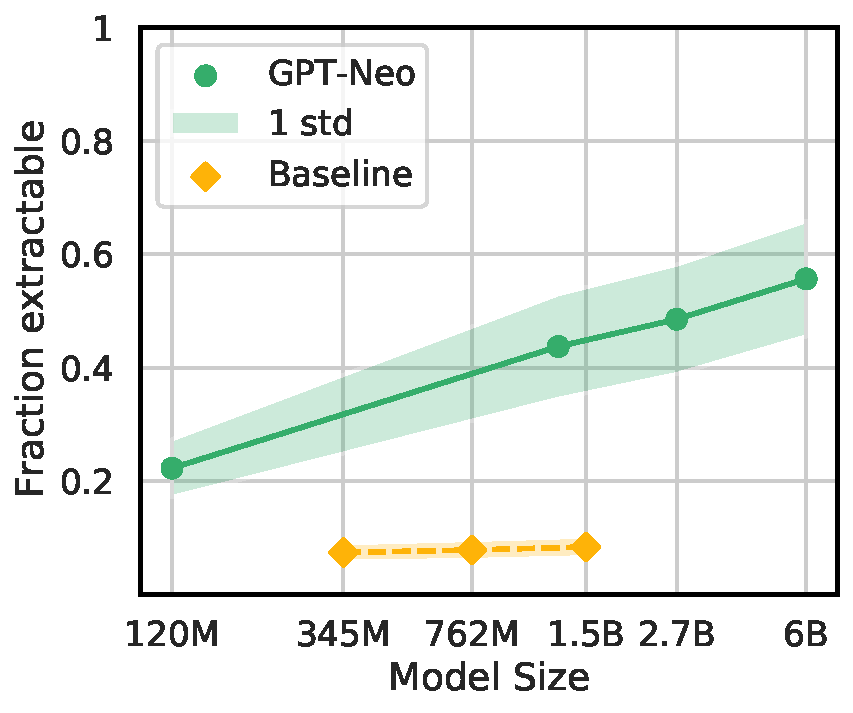
\includegraphics[height=12.2em]{figures/exactly_mem-vs-model_size-prompt-all-gen-50-xlabel-ylabel.pdf} %[height=10.5em]
        %\put(0,-7){(a)}
        % \caption{Model scale}
        \caption{}
        \label{fig:main-res-size}
    \end{subfigure}
    %\hfill
    \hspace{4em}
    \begin{subfigure}[b]{0.27\textwidth}
        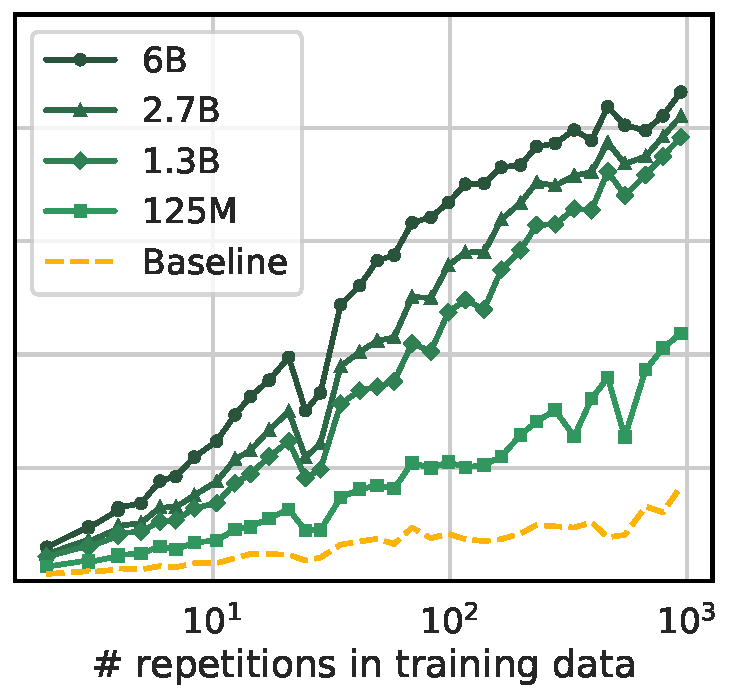
\includegraphics[height=12em]{figures/exactly_mem-vs-repetitions-mean-xlabel-markers.pdf} %[height=10.75em]
        %\put(0,-7){(b)}
        % \caption{Data repetition}
        \caption{}
        \label{fig:main-res-dups}
    \end{subfigure}
    %\hfill
    \hspace{1.7em}
    \begin{subfigure}[b]{0.27\textwidth}
        %\raisebox{3pt}{
        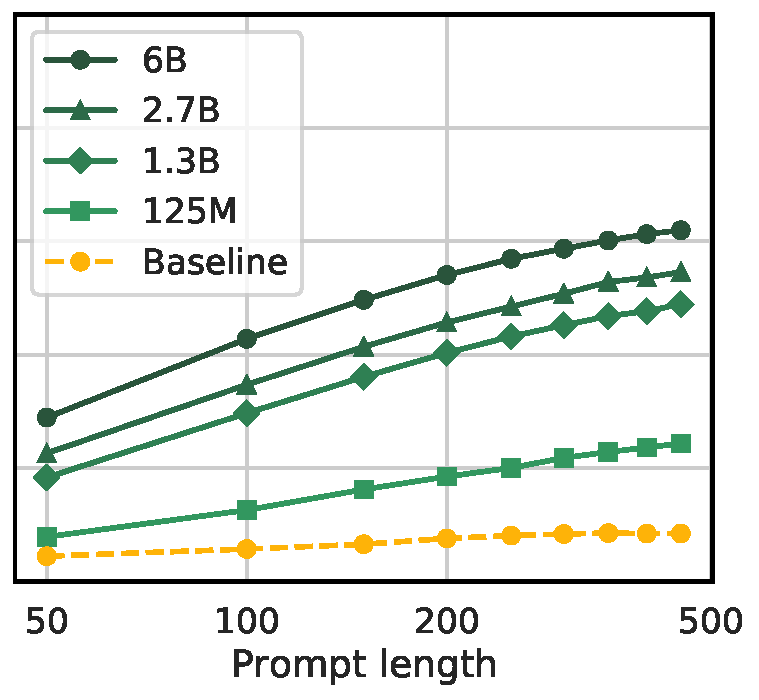
\includegraphics[height=12em]{figures/exactly_mem-vs-prompt_len-seq-500-gen-50-xlabel-markers.pdf} %[height=10.5em]
        %}
        %\put(0,-7){(c)}
        % \caption{Context size}
        \caption{}
        \label{fig:main-res-context}
    \end{subfigure}
    \vskip-5pt
    \caption{
%    \kl{Experiments done on GPT-Neo, then baseline done on GPT2. (baseline, instead of GPT2)}
    We prompt various sizes of GPT-Neo models (green) with data from their training set---The Pile. 
    As a baseline (yellow), we also prompt the GPT-2 family of models with the same Pile-derived prompts, even though they were trained on WebText, a different dataset.
    % because the GPT-2 models were trained on WebText and assuming no overlap between The Pile and WebText, they ``memorized'' examples here represent examples that are easy to generate exact continuations for.
    % We measure the \emph{fraction of extractable examples} as the fraction of model generations that exactly match the true continuation for their prompt.
    \textbf{(a)}
    Larger models memorize a larger fraction of their training dataset, following a log-linear relationship.
    This is not just a result of better generalization, as shown by the lack of growth for the GPT-2 baseline models.
    % The dark shaded region is one std away from the mean, and the lighter shaded region represents the min and max over all document lengths.
    \textbf{(b)}
    Examples that are repeated more often in the training set are more likely to be extractable,
    again following a log-linear trend (baseline is GPT-2 XL). 
    %Varying the number of repetitions results in a log-linear trend with the extraction probabilities.
    % For example, at 5 repetitions, extractability is roughly 8\% for the 1.3B parameter model, while at 35 repetitions, extractability increases to nearly 30\%.
    % \label{fig:duplicates}
    \textbf{(c)}
    As the number of tokens of context available increases, so does our ability to extract memorized text.
    %Increasing the available context from $50$ tokens to $450$ tokens increases
    %the extractability by a factor of \todo{matthew fill in?}
    %For (a) and (b), the fraction extractable is computed over every prompt and sequence length tested.
    % \label{fig:main-res}
    }
    \label{fig:main-res}
\end{figure*}

\subsection{Definition of Memorization}
\label{sec:mem-def}
% In order to evaluate how much a model memorizes, we must first settle on a definition of memorization.
In order to answer the question
``how does $X$ impact memorization?'',
we first select a precise definition for memorization:

%
\begin{definition}
A string $s$ is \emph{extractable with $k$ tokens of context} from a model $f$ if there exists a (length-$k$) string $p$, such that the concatenation $[p \mid \mid s]$ is contained in the training data for $f$, and $f$ produces $s$ when prompted with $p$ using greedy decoding.
\label{def:extractable}
\end{definition}

For example, if a model's training dataset contains the sequence \textit{``My phone number is 555-6789''},
and given the length $k=4$ prefix \textit{``My phone number is''}, the most likely output is \textit{``555-6789''}, then we call this sequence extractable (with 4 words of context).
%
We focus on greedy sampling in this paper, and verify in Section~\ref{sec:modelsize} that our choice of decoding strategy does not significantly impact our results.

While prior work uses other definitions of memorization, we prefer our definition in this paper for several reasons.
%
The first is that it is more actionable.
%
There is a class of memorization definitions, including lower-bounds on differential privacy~\citep{dwork2006calibrating, jagielski2020auditing, nasr2021adversary} or counterfactual memorization~\citep{feldman2020neural, zhang2021counterfactual}, which require training hundreds or thousands of models to measure privacy, 
making them impractical for evaluating enormous language models. 

Other memorization definitions considered for large language models have weaknesses that Definition~\ref{def:extractable} does not. 
Computing \emph{exposure} \citep{carlini2019secret} requires thousands of generations per sequence, and is designed for carefully crafted training examples, making it computationally infeasible for large-scale experiments.
Exposure was also designed to be highly related to the ability of an adversary to extract specific training samples, and we choose to directly measure extractability with access to the entire training set.
Additionally, $k$-eidetic memorization \citep{carlini2020extracting}, where an example is considered $k$-eidetic memorized if it is extractable from the model and appears in at most $k$ examples in the training set,
is a useful definition for \emph{unprompted} memorization, but less useful for memorization when prompting with training data (as we will do).

We are not claiming the definition of memorization used in this section is better for arbitrary privacy measurement
studies.
We use this definition because, when given access to the model's training dataset, ``extractable with $k$ tokens of context''
is a helpful and precise definition.

\subsection{Selection of Evaluation Data}

Having chosen a definition, we next describe our evaluation procedure.
% Having chosen a definition, it next becomes necessary to choose
% a method to evaluate a models' memorization of the training data.
%
Ideally, we would consider every sequence $x=[p \mid \mid s]$ contained in the model's training dataset (where $x$ has been split into a length-$k$ prefix $p$ and a suffix $s$). For each sequence, we would report if the model exactly reproduces $s$ when prompted with $p$, following Definition \ref{def:extractable}.
Unfortunately, performing this test on every sequence in the training data would be prohibitively expensive.
For example, the largest 6 billion parameter GPT-Neo model has a throughput of roughly one 100-token generation per second on a V100 GPU. Extrapolating to the 800GB training dataset, this would require over $30$ GPU-years of compute.

Instead, we query on a small subset of the training data.
%
This subset should be small enough that it is feasible to test for extraction, 
but also large enough that
it gives statistical confidence.
%
In this paper we choose subsets of roughly $50{,}000$ sequences.
%\footnote{Even at this low number of sequences, the generations analyzed in this paper still require 
%over $1{,}000$ GPU-hours of compute.}
The primary criteria when choosing a subset of the training data is to obtain a representative sample that allows
us to draw meaningful conclusions from the data.
%
Yet, naively sampling from the data independently at random to construct a representative subset of the data distribution is not the best approach.
Indeed, prior work has identified that one of the most important factors that contributes to training data memorization is how often that data has been \emph{duplicated} (i.e., how often the same sequence is repeated either exactly or approximately-exactly).
%
Because the frequency of training data duplication follows an exponential distribution \citep{lee2021deduplicating}, a fully random sample of only 50,000 sequences
(accounting for $\le 0.02\%$ of the dataset)
is unlikely to contain \emph{any} signal that would allow us to 
accurately measure the tail of this distribution.




Instead, we construct a duplication-normalized subset.
%
For each sequence length $\ell \in \{50,100,150,\dots,500\}$,
and integer $n$,
we select 1,000 sequences of length $\ell$ that are contained in the training dataset between $2^{n/4}$ and $2^{(n+1)/4}$ times.
We do this until we reach an $n$ for which 1,000 sequences are not available.
%
This gives us $1000$ sequences that repeat between $6$ and $8$ times ($\approx 2^{11/4}$ and $\approx 2^{12/4}$) and also $1000$ sequences that repeat between $724$ and $861$ times ($\approx 2^{38/4}$ and $\approx 2^{39/4}$).
%
This biased sampling allows us to more accurately measure memorization as a function of a sample's duplication factor, without querying the entire dataset.
%
Note that constructing this duplicate-normalized data subset requires some work,
as efficiently identifying duplicate substrings in an $800$GB training dataset is
computationally challenging.
%
We make use of the suffix array construction from \citet{lee2021deduplicating} (see Appendix).

For each sequence length between $50$ and $500$ tokens, this collection process gives us roughly $50,000$ examples duplicated varying numbers
of times,
totaling roughly $500{,}000$ sequences.
%
For each length $\ell$ sequence, we prompt the model with the first $\ell-50$ tokens and report the sequence
as ``extractable'' if the next $50$ tokens emitted by the model exactly match the $50$ token suffix of this sequence.
Fifty tokens corresponds to an average of 127 characters or 25 words\footnote{As measured by \href{https://spacy.io/}{spaCy} on the GPT-Neo training set.}, well over the length of a typical English sentence.
%
Finally, we compute the average probability that a sequence is extractable by averaging over all lengths $\ell$.


\subsection{Experiments}

\subsubsection{Model and Dataset}
We primarily study the GPT-Neo model family~\citep{gpt-neo,gpt-j} trained on the Pile dataset~\citep{gao2020pile}.
The GPT-Neo models are causal language models 
trained with the objective of predicting the next token in a sequence given the previous ones.
They come in four sizes: $125$ million, $1.3$ billion, $2.7$ billion and $6$ billion parameters. 
The Pile is a dataset containing text collected from various sources (e.g., books, Web scrapes, open source code) that totals $825$GB.
%
The largest GPT-Neo model is the largest language model available for public download, and The Pile is the largest public text dataset available.

\subsubsection{Bigger Models Memorize More}
\label{sec:modelsize}
We begin by considering the impact of model size on memorization,
expanding on prior studies which qualitatively established a relationship between the size of GPT-2 models and their
ability to memorize $<$30 URLs \citep{carlini2020extracting}.
% As mentioned earlier, prior work has shown qualitative relationships between model size and
% memorization ability (e.g., by showing that larger GPT-2 models memorize a few more URLs (suspected to be in the GPT-2 training dataset) than smaller models \citet{carlini2020extracting}).
%
In contrast, we study \emph{a million} model generations in order to describe
how model scale relates to memorization.

\paragraph{Results.}
The results of this experiment are given in Figure~\ref{fig:main-res-size}.
%
The y-axis reports the fraction of generations which exactly reproduce the true suffix for their prompt, averaged over all prompt and sequence lengths we experimented on.
%
We find that larger models memorize significantly more than smaller models do, with \emph{a near-perfect log-linear fit} ($R^2$ of 99.8\%): a ten fold increase in model size corresponds to an increase in memorization of 19 percentage points.\footnote{This trend cannot continue indefinitely; the maximum percentage is 100\%.
We do not address these complications as our results max out at $\sim$60\%, but future work may need to handle these additional difficulties when extrapolating to even larger models.}

To confirm that larger models are indeed \emph{memorizing} more data, and not simply \emph{generalizing} better, we also perform the same analysis with the GPT-2 model family as a baseline. 
%
The GPT-2 family of models are similarly sized, and also trained on Internet-scraped data.
If our ``larger models memorize more'' results were due to the general predictive strength of larger models, and not the memorization of specific training data, we would expect a similar relationship between comparably sized GPT-2 models trained on similar data. 
%
Put differently, this baseline allows to establish
what fraction of the training data is sufficiently ``easy'' that any language model could correctly
predict the 50-token suffix, even if the example had never been seen before during training.
For example, a language model that has seen multiple examples of number sequences during training could learn to correctly complete other number sequences that were not seen in training.
%
%Any intersection between GPT-2 and GPT-Neo training sets will overestimate GPT-2's completion rate, making memorization appear less frequently.
%

We find that approximately $6\%$ of the examples in our evaluation dataset can be correctly 
completed by GPT-2, compared to $40\%$ for a similarly sized 1.3B parameter GPT-Neo model. 
A qualitative analysis (see examples in Appendix Figure~\ref{fig:egs-mem-by-gpt2}) suggests that examples ``memorized'' by GPT-2 are largely uninteresting
sequences (e.g., number sequences, repetitions of the same few tokens, or common phrases).
%
Therefore, we conclude that when larger models have a higher fraction of extractable training data,
it is because they have memorized the data; it is not simply because the larger models are generally more accurate.


\subsubsection{Repeated Strings are Memorized More}
\label{sec:duplicates}
Prior work has provided preliminary evidence that memorization in language models increases with the number of times sequences are repeated in the training set \citep{carlini2020extracting, lee2021deduplicating}.
%
We expand on this observation and systematically measure the effect number of repetitions has on memorization.
%
Using our experimental methodology, we measure the fraction of sequences which are extractable, for sequences in each bucket of duplicate counts, varied between 2 duplicates and 900 duplicates.
Each bucket consists of $1{,}000$ distinct sentences, and we compute the average amount of memorization for each bucket.


\paragraph{Results.}
Figure~\ref{fig:main-res-dups} shows an analysis of our results, aggregated over all sequence lengths.
We find a clear log-linear trend in memorization. While the model struggles to regurgitate strings which are repeated just a handful of times, this probability increases dramatically as strings have more repetitions.
%
%Strings repeated only once are memorized by the 1.3B parameter model with probability $TODO$, and even at 5 repetitions this probability is still only 8\%. 
These small memorization values at low numbers of repetitions corroborate the impact of training dataset deduplication on memorization observed by \citet{lee2021deduplicating}.
%
However, we find that memorization does still happen, even with just a few duplicates---thus, deduplication will not perfectly prevent leakage.
%
While this relationship is perhaps obvious, and has been corroborated for specific training examples in prior work \citep{carlini2019secret, carlini2020extracting}, our results show that it holds \emph{across the entire training set}.


\subsubsection{Longer Context Discovers More Memorization}
\label{sec:context}
The previous two questions evaluated how data collection and model training decisions impact the leakage of a model's training data when it is provided a fixed number of tokens from a sequence as context.
As a result, those experiments suggest particular actions that could be taken to mitigate memorization (by reducing model size, or limiting the number of duplicate examples).

However, even when the model is fixed, it is possible to vary the amount of extractable training data by controlling the length of the prefix passed to the model. 
By studying how the number of tokens of context impacts extractability, we demonstrate the difficulty of \emph{discovering} memorization---language models may only exhibit their memorization under favorable conditions.


\paragraph{Results.}
In Figure~\ref{fig:main-res-context}, we observe that the fraction of extractable sequences increases log-linearly with the number of tokens of context. For example, 33\% of training sequences are extractable from the 6B model at 50 tokens of context, compared to 65\% with $450$ tokens of context.

% We call this the \textbf{extractibility phenomenon}:
We call this the \textbf{discoverability phenomenon}:
some memorization only becomes apparent under certain conditions, such as when the model is prompted with a sufficiently long context.
This makes ``discovering'' memorization difficult.

% with sufficient prompting, current models extensively memorize their training datasets, but it is not easy to discover that this memorization has occurred.
% The models only exhibit memorization of some sequences when given sufficient context.
%
%Here, the model might not be able to give the correct answer, despite the fact that
%the model could know the answer if only more context were available.

The discoverability phenomenon may seem natural: conditioning a model on $100$ tokens of context is more specific than conditioning the model on $50$ tokens of context, and it is natural that the model would estimate the probability of the training data as higher in this situation. 
However, the result is that some strings are ``hidden'' in the model and require more knowledge than others to be extractable.

From one point of view, it is good that some memorization is difficult to discover.
This makes it harder for attackers to perform training data extraction attacks \citep{carlini2020extracting},
or otherwise exploit memorization.
Indeed, if an exact $100$ token prompt is required to make the model output a given string, then, in practice, an adversary will likely be unable to perform the attack.
%
The difficulty in discovering memorization also reduces the likelihood of \emph{non-adversarial} training data regurgitation.
For example, the GitHub CoPilot model~\citep{chen2021evaluating} reportedly rarely emits memorized code in benign situations, and most memorization occurs only when the model has been prompted with long code excerpts that are very similar to the training data~\citep{ziegler2021copilot}.
Practitioners building language generation APIs could (until stronger attacks are developed) significantly reduce extraction risk by restricting the maximum prompt length available to users.

Viewed differently, however, the difficulty of discovering memorization
can also harm our ability to audit privacy in machine learning models.
%
Because existing approaches for provably-correct privacy-preserving training of machine learning are applied only rarely in practice~\citep{abadi2016deep, thakkar2020understanding, ramaswamy2020training},
it is common to attempt post-hoc \emph{privacy auditing}~\citep{jayaraman2019evaluating, jagielski2020auditing, nasr2021adversary}.
%
Our results suggest that correctly auditing large language models will likely require prompting the model with training data, as there are currently no known techniques to identify the tail of memorized data without conditioning the model with a large context.
%
Improving upon this limitation is an interesting problem for future work.


\begin{figure}
    \centering
    \begin{subfigure}[a]{0.34\textwidth}
        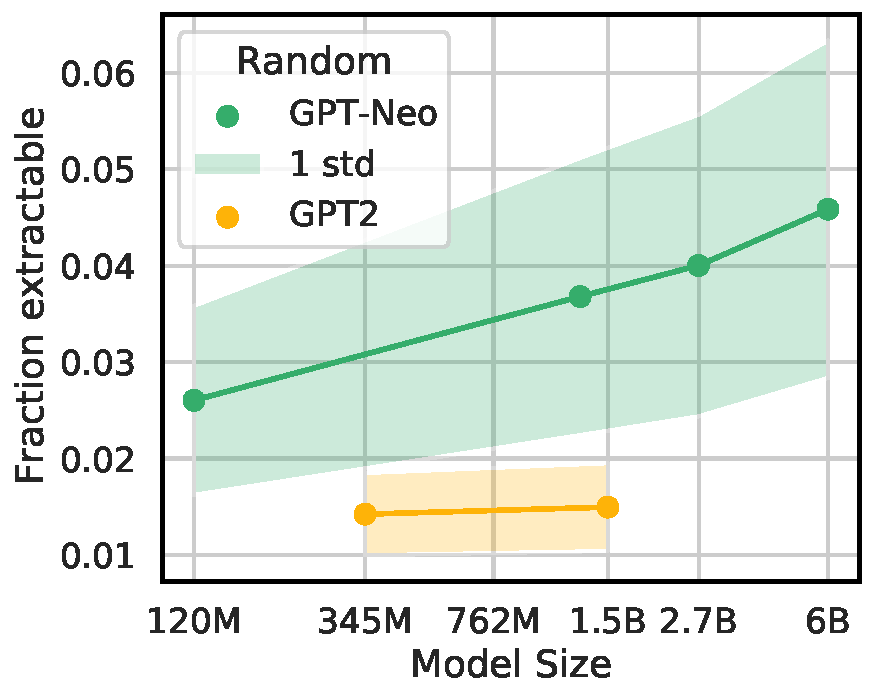
\includegraphics[width=\textwidth]{figures/random-exactly_mem-vs-model_size-prompt-all-gen-50-xlabel-ylabel} %[height=10.75em]
        %\put(0,-7){(b)}
        % \caption{Model Scale}
        \caption{}
        \label{fig:other_approaches_randomsize}
    \end{subfigure}
    \hfill
    \begin{subfigure}[a]{0.34\textwidth}
        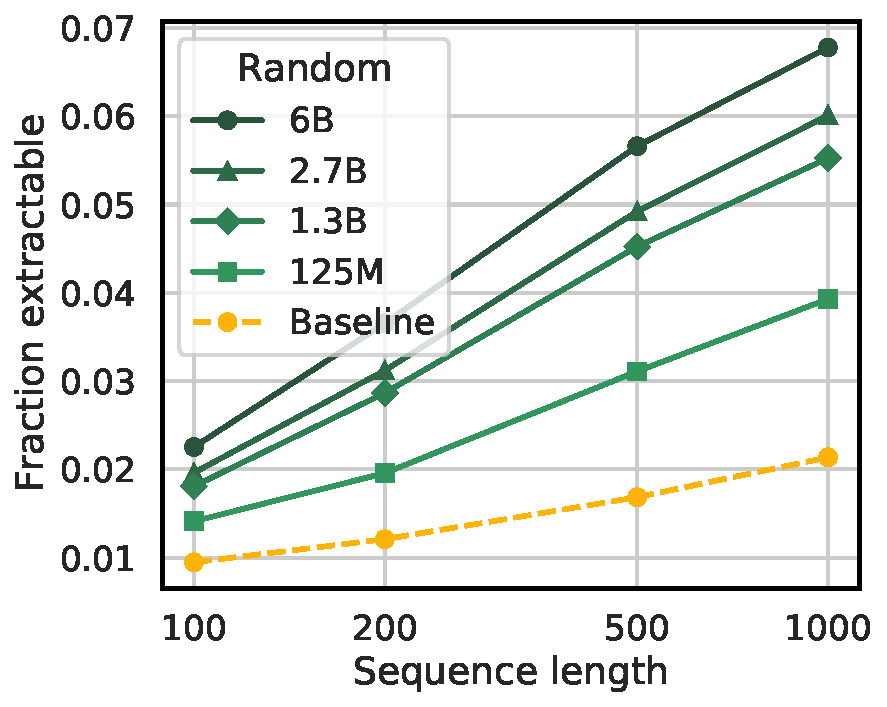
\includegraphics[width=\textwidth]{figures/random_exactly_mem-vs-prompt_len-seq-varyseqlen-gen-50-xlabel-ylabel-markers} %[height=10.75em]
        %\put(0,-7){(b)}
        % \caption{Sequence length}
        \caption{}
        \label{fig:other_approaches_randomlength}
    \end{subfigure}
    % \begin{subfigure}[a]{0.16\textwidth}
    %     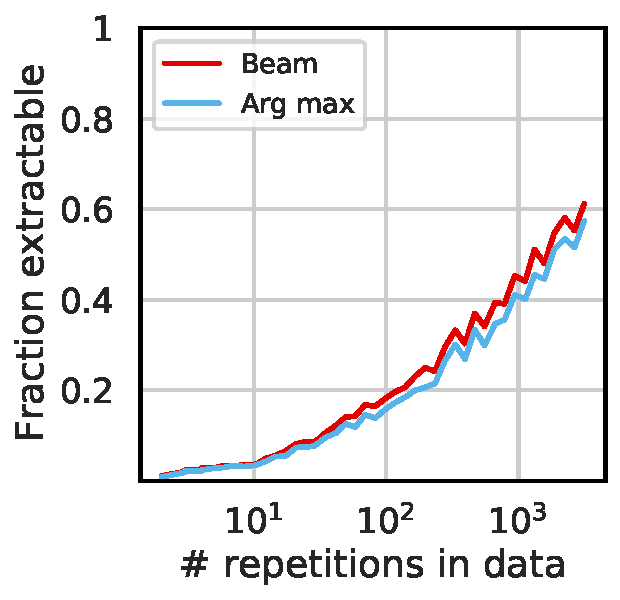
\includegraphics[width=\textwidth]{figures/beam_search} %[height=10.5em]
    %     %\put(0,-7){(a)}
    %     \caption{Decoding strategy}
    %     \label{fig:other_approaches_decoding}
    % \end{subfigure}
    % \begin{subfigure}[a]{0.16\textwidth}
    %     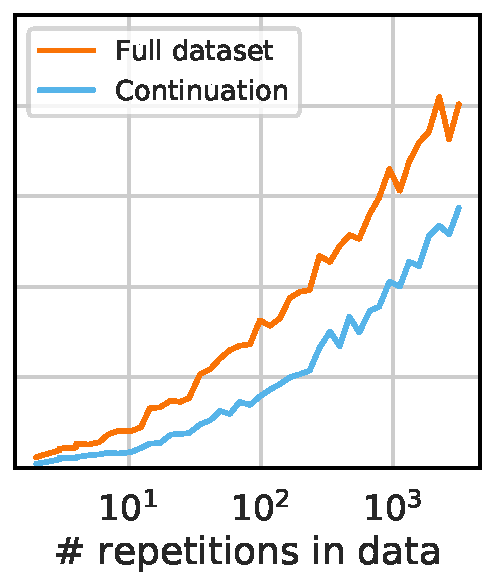
\includegraphics[width=\textwidth]{figures/overall} %[height=10.75em]
    %     %\put(0,-7){(b)}
    %     \caption{Search strategy}
    %     \label{fig:other_approaches_search}
    % \end{subfigure}
    \hfill
    \begin{subfigure}[a]{0.3\textwidth}
        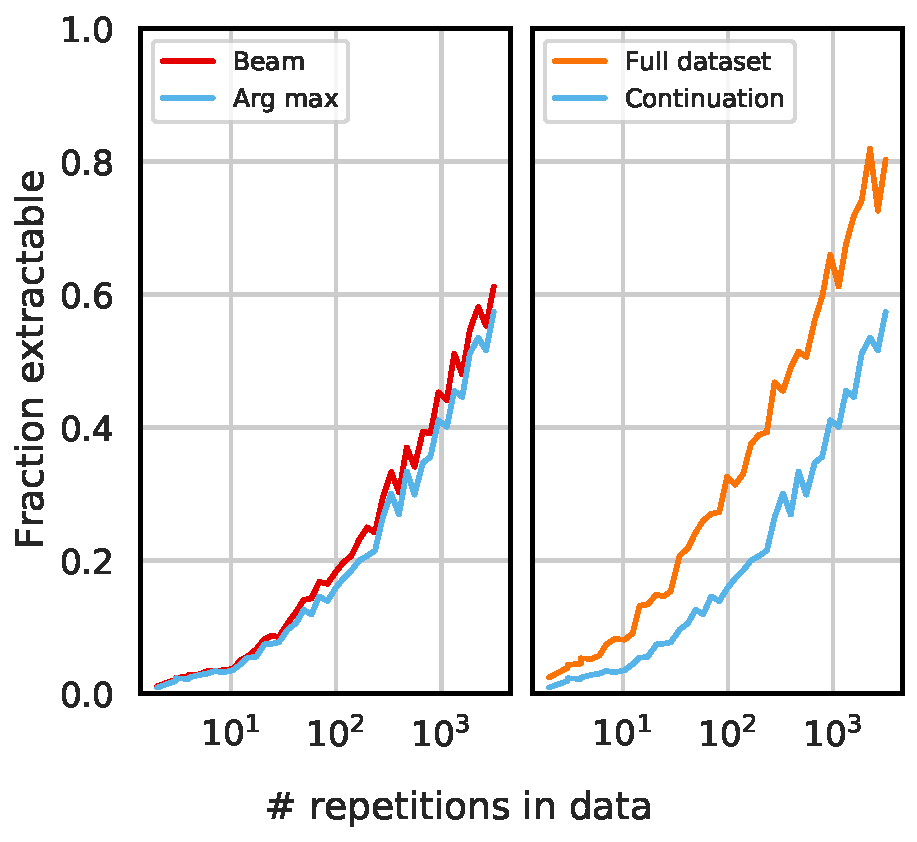
\includegraphics[width=\textwidth]{figures/beam_search_and_overall} %[height=10.75em]
        %\put(0,-7){(b)}
        % \caption{Decoding and search strategies}
        \caption{}
        \label{fig:other_approaches_search}
    \end{subfigure}
    
    \vskip-5pt
    
    \caption{
    \textbf{(a)} Percentage of sequences extracted as a function of model scale where we sample randomly from the training set. 
    \textbf{(b)} Percentage of sequences extracted as we vary the length of the prompt. For each sequence length $n$, $n$-50 tokens are used as the prefix, and we check for extraction of the remaining 50 tokens.
    \textbf{(c-left)} Using beam search with $b$=100 slightly increases the data extracted. \textbf{(c-right)} We observe considerably more memorization when checking whether the generated sequence occurs anywhere in the entire training set (Section \ref{section:other_approaches}). However, this approach is very computationally expensive so we do not use it for experiments.}
    \label{fig:other_approaches}
\end{figure}

\subsubsection{Alternate Experimental Setting: Random Dataset Sampling}

\label{section:other_approaches}
The majority of this paper uses subsets of the training data that were explicitly sampled according to training data duplication frequency.
%
We now explore what would happen if we instead choose a
truly random subset of the training data, where each sequence is sampled uniformly.
%
Specifically, we randomly sample $100,000$ sequences
from The Pile dataset of length 100, 200, 500, and 1000;
prompt the model with the first $N-50$ tokens; and then
test for memorization by verifying if the model can emit the remaining $50$ tokens perfectly.    
%
We explore the result of this analysis in
Figure~\ref{fig:other_approaches_randomsize} and Figure~\ref{fig:other_approaches_randomlength}.
We again vary the size of the models we train and the
context length we provide to understand how this impacts memorization---but this time through prompting the models
with randomly sampled training sequences.
%
As expected, the absolute probability of memorization is much lower than in Figure~1 where we prompted models with training data from the sampled duplication-normalized subset.

As before, we observe similar trends with model scale and context length.
Larger models memorize more training examples than smaller models---and much more than the baseline GPT-2 model
that was not trained on The Pile.
%
Similarly, providing more context to a model increases
the likelihood we can discover memorization.
%
In Figure~\ref{fig:other_approaches_randomlength}, we prompt models with: $\text{prompt length} = \text{sequence length} - 50$. We see that the longer prompts are easier to predict correctly than shorter prompts. 
% Here, however, we find that longer sequences \emph{are}
% easier to predict correctly than shorter sequences:
The baseline GPT-2 model is nearly twice as accurate on
sequences of length $1000$ (prompt length $ = 950$) compared to sequences of length $100$ (prompt length $ = 50$).
%

We can extract the last 50 tokens of
a length-1000 sequence with nearly $7\%$ probability
for the largest GPT-J 6B model compared to $4\%$ probability 
for the smallest $125$M GPT-Neo model. (And both
of these are much larger than the $2\%$ probability 
of extraction for the $1.5$B parameter GPT2-XL model.)
%
These results taken together allow us to establish an estimated lower bound that
there is $1\%$ of The Pile dataset that is extractable
by the 6B GPT-J model, but not by GPT-2 XL.


\subsubsection{Alternate Experimental Setting: Beam Search Decoding}
We previously defined memorization as the ability of a model to generate the true continuation when the \emph{most likely} token is chosen at every step of decoding.
However, this greedy decoding strategy does not produce the overall most likely sequence.
Many language model applications use other decoding strategies, such as beam search (an algorithm for efficiently searching over the exponential space of sequences that could possibly be generated) to find the one with highest possible likelihood.
To understand how our choice of decoding strategy affects the amount of memorization we measure, we compare greedy decoding with beam search in Figure \ref{fig:other_approaches}(c).

We find that using beam search (with $b = 100$) results in only slightly more extracted memorization.
The average difference in fraction of extractable memorization is just under 2 percentage points on average, with a maximum of 5.6. %, for the bucket containing sequences with about 1300 repetitions, and the average difference is around $2\%$.
Interestingly, beam search and greedy decoding generated the same output 45\% of the time.

The most common decoding strategy employed by modern LMs is \emph{random sampling}, where the next token is selected at random according to a probability distribution derived from the model's predictions.
\citet{mccoy2021raven} found that random sampling resulted in generated text with a greater number of novel $n$-grams.
Since the goal of our study is to maximize discoverability---an antithetical goal to maximizing linguistic novelty---we do not present experiments that use random sampling.

\begin{figure*}
    \centering
    %### two row version
    %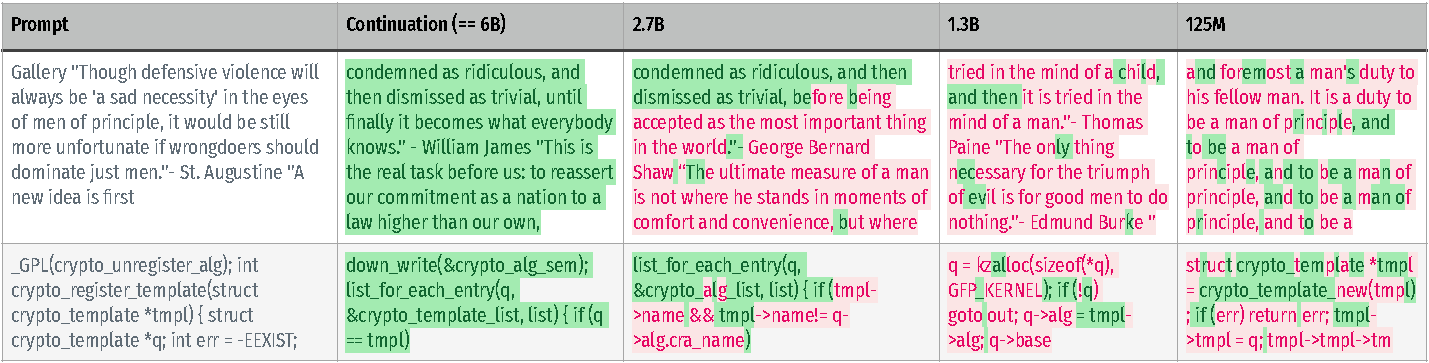
\includegraphics[width=\linewidth]{figures/text-egs/style2-mem-by-6B_pg4.pdf}
    %### three row version
    %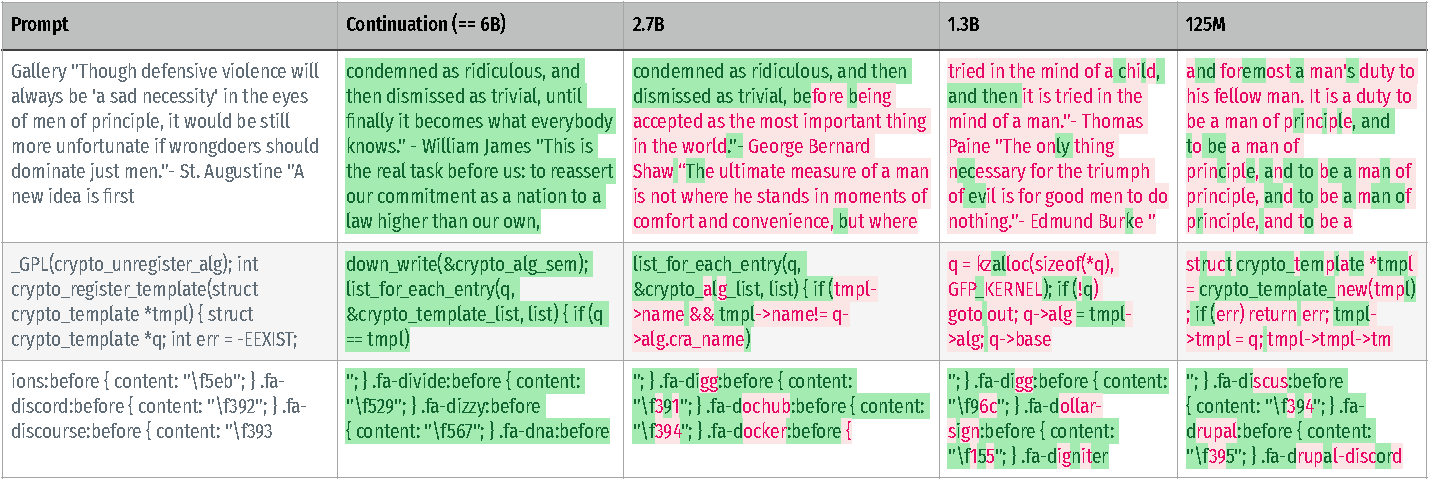
\includegraphics[width=\linewidth]{figures/text-egs/style2-mem-by-6B_pg5.pdf}
    %### four row version
    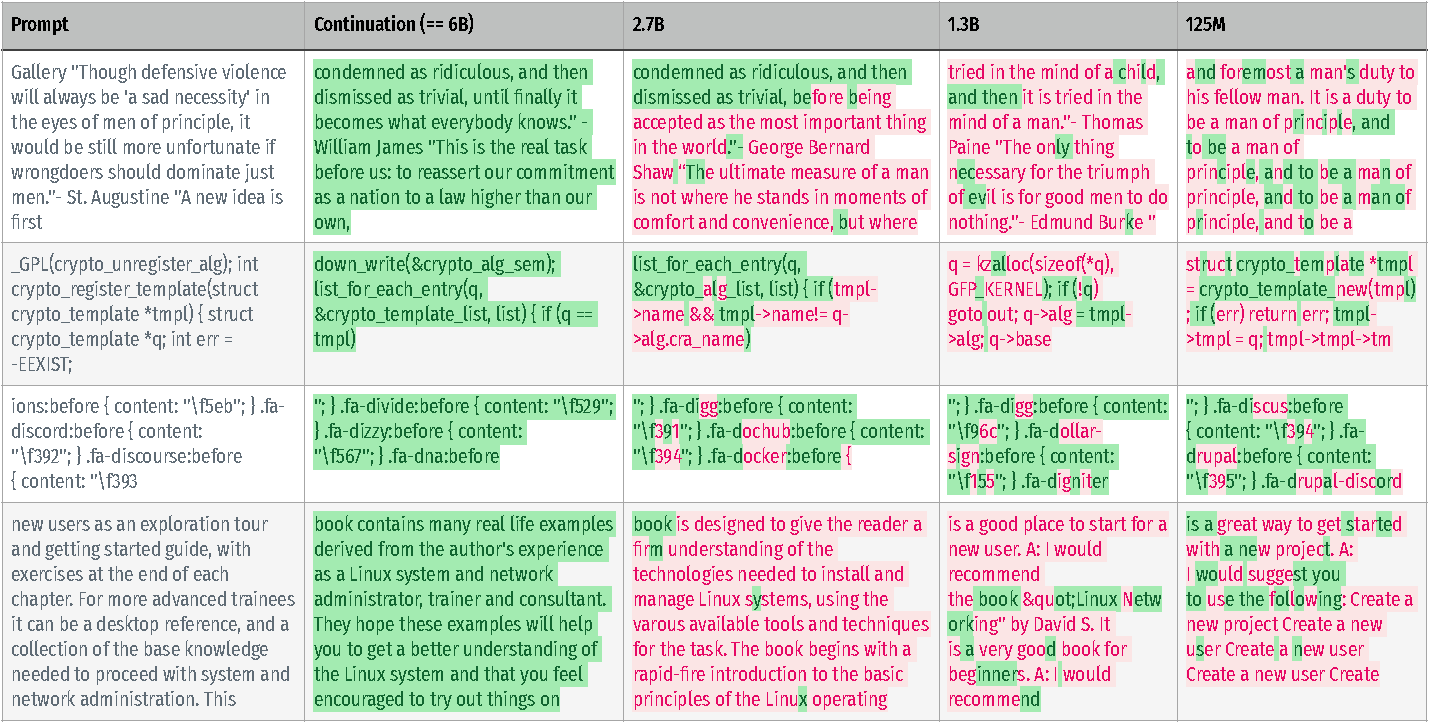
\includegraphics[width=\linewidth]{figures/text-egs/style2-mem-by-6B_pg6.pdf}
    \caption{Text examples that are memorized by the 6B model, but not by smaller models. Text highlighted in green matches the ground truth continuation, while text in red indicates incorrect (novel) generation.}
    \label{fig:egs-mem-by-6b-body}
    
    
\end{figure*}

\subsubsection{Alternate Definition of Extractability}
Our main experiments report a sequence as ``extractable'' if the model's generated continuation is identical to the true suffix within that training example.
This method is a loose lower bound on memorization.
Consider two sequences $x_1$, $x_2$ both contained in the training dataset.
Suppose these two sequences share the same prefix, and differ only in the final suffix;
that is, $x_1 = [p || s_1]$ and $x_2 = [p || s_2]$.
When we select $x_1$ and prompt the model on the prefix $p$, we will 
report ``success'' \emph{only if the output equals $s_1$}, but not if the output is $s_2$,
even though this is \emph{also} a form of memorization.
%

We now consider how our results would change if we instead checked that the generation $[p || f(p)]$ from a prompt $p$ was contained \emph{anywhere} in the training dataset. This gives a strictly larger measurement of memorization.
By comparing these two methods (checking for memorization within the ground truth continuation, and within the entire dataset), we can understand how the choice of measurement affects the results in our experiments. 


% Here we consider an alternative, more general method for measuring memorization that accounts for shared prefixes.
% When instead of declaring a successful, we prompt the model with the sequence $p$
% extraction only if the true suffix is produced, we could check if the sequence $[p || f(p)]$
% is contained \emph{anywhere} in the training dataset.
% This methodology will give a strictly larger measurement of memorization.

Searching within the entire dataset finds more memorized content than comparing with the ground truth (Figure \ref{fig:other_approaches_search}). 
For examples at 100 repetitions $32.6\%$ of outputs are contained somewhere in the dataset but just $15.8\%$ match the ground truth continuation.
This difference becomes more pronounced as the number of repetitions increases. 
The maximum difference between these approaches is 28.4\%, at 2{,}200 repetitions.
%difference between searching the entire dataset vs. comparing with the continuation is $28\%$ 
%(0.2839999999999999, 2234.016)

We refrain from using this approach for our main experiments,
%First, studying repetition in internet datasets requires understanding how so many repetitions of an example came to be. 
%There are many approximate duplicates such as those containing text generated from templates~\cite{lee2021deduplicating}.
%Thus, $80\%$ memorization when checking in the entire dataset and also nearly $60\%$ memorization when comparing with the groundtruth are both not as concerning as the raw numbers might suggest.
%
% First, the total gap between the two methodologies is rather small---this improvement
% finds an additional \TODO{\%} of memorization instances not found previously.
%
because this definition requires vastly larger computation resources; it requires
querying whether hundreds of thousands of sequences are contained in an 800GB
training dataset.
%
Therefore, to promote reproducability, the remainder of this paper continues with testing the generated suffix against the single expected training suffix.
% And while we have developed special suffix-array tooling to perform this computation efficiently,
% in order to allow our work to be more easily reproduced, we TODO our main methodology
% that only requires a simple equality test between two length-50 sequences.
%
% (Nevertheless, we believe that it is important to have verified this methodology is
% indeed sufficient---if this new approach had given dramatically different results, 
% it may have been necessary to apply this more general approach.)

\subsubsection{Qualitative Examples of Memorization}

\begin{table}[t]


    \small
    \begin{tabular}{@{} l r r r r r @{}}
        \toprule
            &&  \multicolumn{4}{c}{Not Memorized By}\\
        \cmidrule{3-6}
         Model & Memorized & 125M & 1.3B & 2.7B & 6B\\
         \midrule
         125M & 4{,}812 &
         - & \cellcolor{blue!2}328 & \cellcolor{blue!1}295 & \cellcolor{blue!1}293\\
         
         1.3B & 10{,}391 &
         \cellcolor{blue!29}5{,}907 & - & \cellcolor{blue!6}1{,}205 & \cellcolor{blue!5}1{,}001\\
         
         2.7B & 12{,}148 &
         \cellcolor{blue!37}7{,}631 & \cellcolor{blue!14}2{,}962 & - & \cellcolor{blue!7}1{,}426\\
         
         6B & 14{,}792 &
         \cellcolor{blue!50}10{,}273 & \cellcolor{blue!26}5{,}402 & \cellcolor{blue!20}4{,}070 & - \\
         \bottomrule
    \end{tabular}
            \centering\caption{The number of sequences memorized by one model, and not memorized by another. Not all sequences memorized by a small model are also memorized by a larger model. As a model gets larger, it memorizes more unique sequences.}\vspace{1em}
    \label{tab:memorized_by_model}
\end{table}

We now turn to inspect the training sequences memorized by the models.\footnote{For these results we sample 50-token prompts, 50-token continuations, and randomly sample across duplication counts.} Figure~\ref{fig:egs-mem-by-all} in the appendix shows examples of sequences that are memorized by \emph{all} the models. We found most of these universally-memorized sequences to be ``unconventional'' texts such as code snippets or highly duplicated texts such as open source licenses. %Note the license texts are memorized verbatim---the asterisks due to C/C++ style comments formatting are reproduced faithfully.

More interestingly, Table~\ref{tab:memorized_by_model} summarizes the total number of sequences that are memorized by
one model but not another.
Increasing model size leads to large numbers of nonoverlapping memorized sequences, although every model has some amount of memorization not shared by each other model.
(Even the $125$M model memorizes a few sequences the $6$B model does not.)

In Figure~\ref{fig:egs-mem-by-6b-body}, we present qualitative examples that are only memorized by the largest (6B) model.
In these examples, the 50-token generations of the 6B model match the groundtruth continuations exactly, but the generations from the smaller models match \emph{neither} the groundtruth continuations of the prompted examples \emph{nor} any other training examples with the same prompts.
We highlight some interesting patterns in these sequences: while the generations from the smaller models do not match the training data, they are generally thematically-relevant and locally consistent. However, a closer inspection reveals that those generations are syntactically sound but semantically incorrect.
Figure~\ref{fig:egs-mem-by-all} lists examples that are memorized by models of \emph{all} sizes, in the sense that the 50-token generations match the groundtruth continuations of the prompts.


In Figure~\ref{fig:egs-mem-by-125M} we show examples that are only memorized by the smallest model, using similar criterion as when we filter examples that are only memorized by the largest model. There are significantly fewer examples that are only memorized by the smallest model (35) than only memorized by the largest model (2860).
The first row of Figure~\ref{fig:egs-mem-by-125M} is particularly interesting: the groundtruth continuation contains a typo due to formatting cutoff.
While the smallest model memorized the typo, larger models try to fix the typo.

In Figure~\ref{fig:egs-mem-but-not-rep} and Figure~\ref{fig:egs-rep-but-not-mem} we show examples that are memorized but not heavily duplicated in the training set, and examples that are heavily duplicated but not memorized, respectively. Finally, we show examples that are memorized by GPT2-XL in Figure~\ref{fig:egs-mem-by-gpt2}.

\begin{figure}
    \centering
    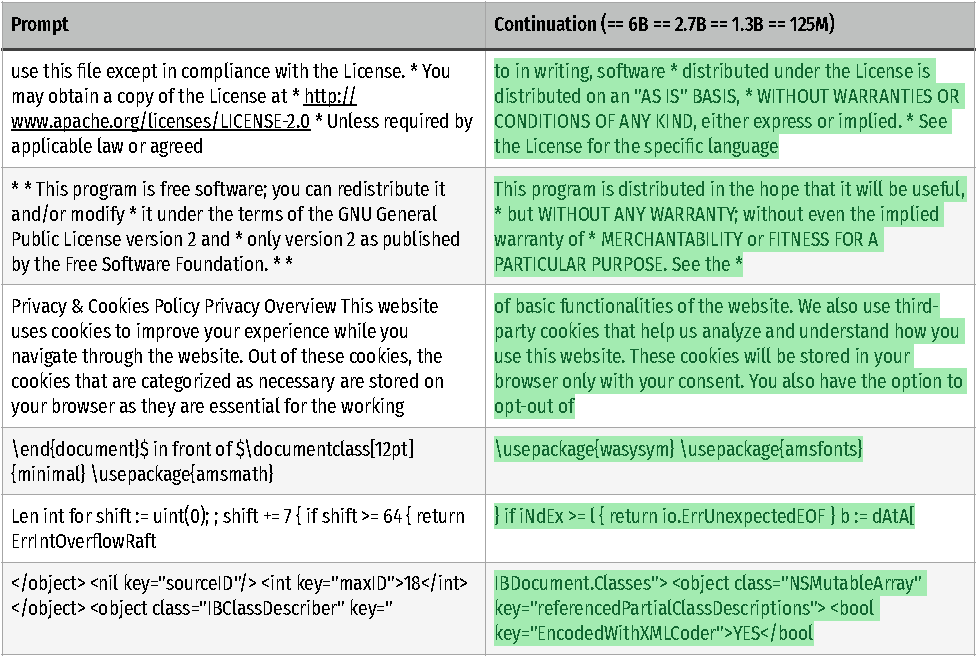
\includegraphics[width=.8\linewidth]{figures/text-egs/style2-mem-by-all_pg1.pdf}
    \caption{Text examples that are memorized by all the models: given 50-token prompts on the left, the next 50 tokens generated by all the models match the groundtruth continuation.}
    \label{fig:egs-mem-by-all}
\end{figure}


\begin{figure}
    \centering
    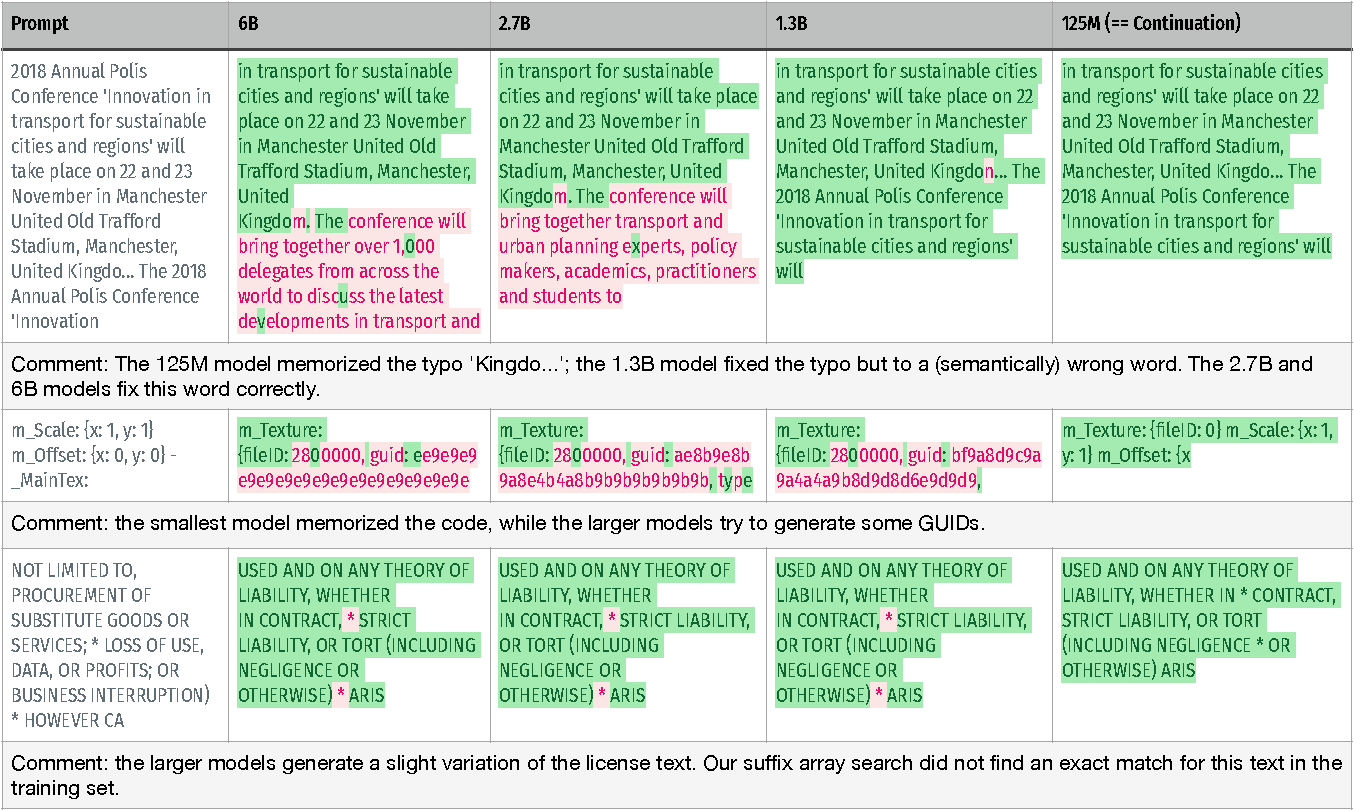
\includegraphics[width=.7\linewidth]{figures/text-egs/style2-mem-by-125M_pg1.pdf}
    \caption{Text examples that are memorized by the 125M model (according to true-continuation match), but not memorized by larger models (the generated texts do not match the true continuation, nor any other training examples). The first column shows the prompt. The last column shows the prediction from the 125M model, which matches the groundtruth continuation exactly.}
    \label{fig:egs-mem-by-125M}
\end{figure}

\begin{figure}
    \centering
    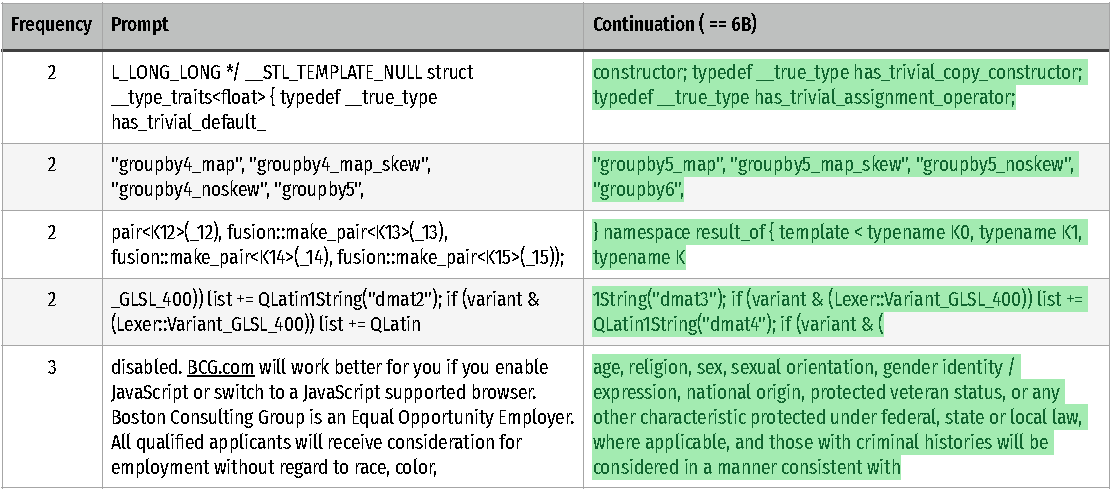
\includegraphics[width=0.7\linewidth]{figures/text-egs/style2-mem-but-not-rep_pg1.pdf}
    \caption{Text examples that are memorized but are not heavily duplicated in the training set. Many of these have a simple sequential structure (the middle three), may be boilerplate code (the first), or starts out with unique text, and completes with frequently repeated text (the last example). Overall, these are easily completed sequences.}
    \label{fig:egs-mem-but-not-rep}
\end{figure}

\begin{figure}
    \centering
    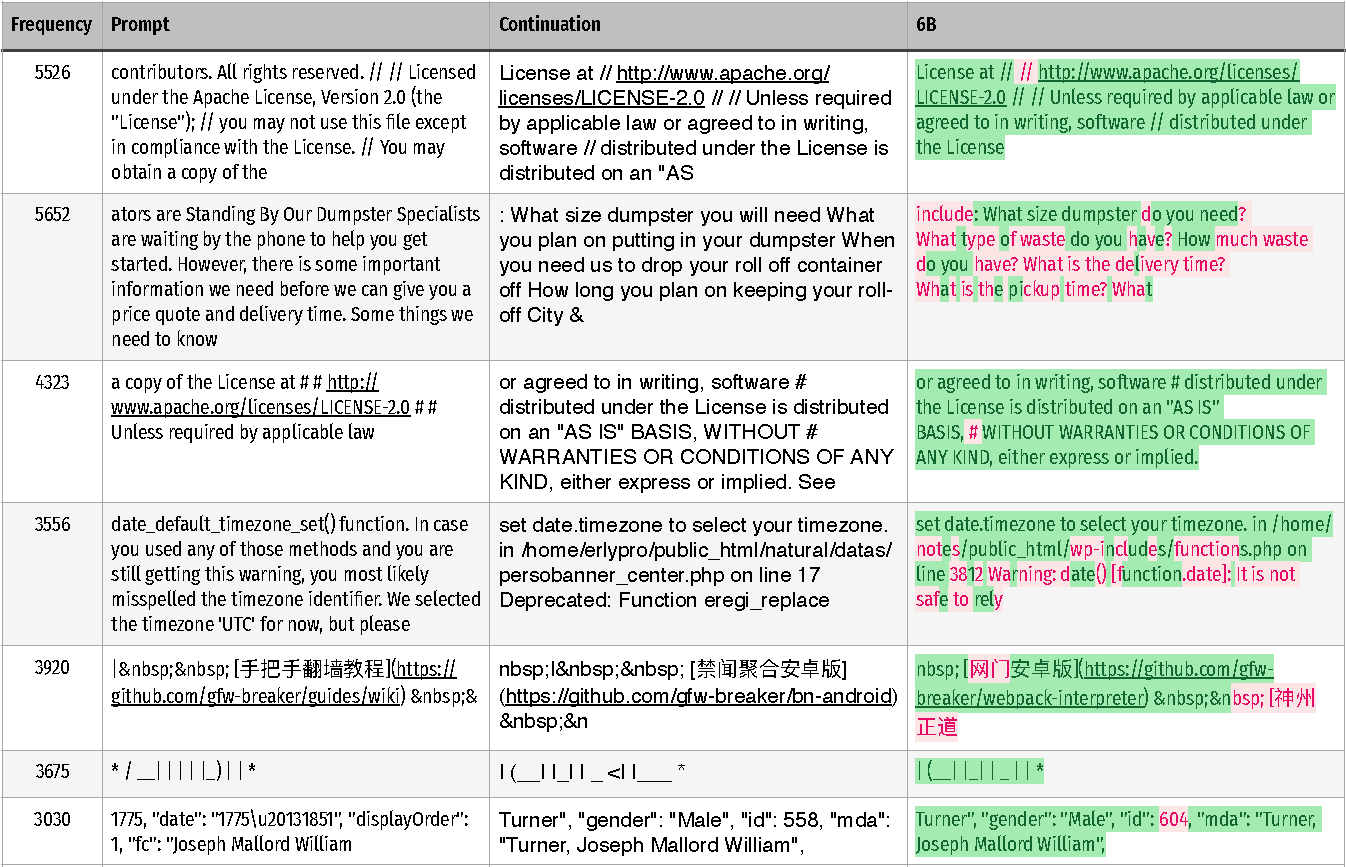
\includegraphics[width=0.7\linewidth]{figures/text-egs/style2-rep-but-not-mem_pg1.pdf}
    \caption{Text examples that are heavily replicated in the training set but not memorized. We find many examples which have slight differences with no semantic (English) meaning. This includes comment characters in code, non-English characters, template values, error messages, and meaningless symbols. We also surprisingly find a large number of slightly different but heavily repeated documents about dumpsters.}
    \label{fig:egs-rep-but-not-mem}
\end{figure}

\begin{figure}
    \centering
    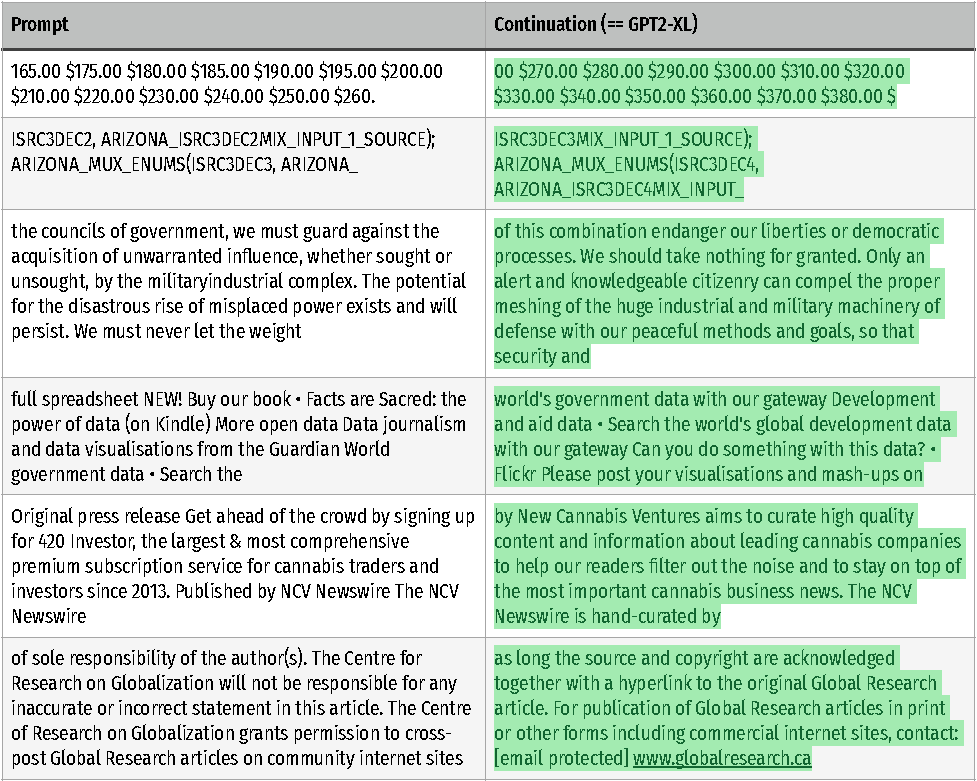
\includegraphics[width=0.7\linewidth]{figures/text-egs/style2-mem-by-GPT2_pg1.pdf}
    \caption{Text examples that are from The Pile and memorized by GPT2-XL. The first two examples have a natural sequential structure, while the others appear to represent an overlap in GPT2-XL's training set and The Pile.}
    \label{fig:egs-mem-by-gpt2}
\end{figure}

% Appendix~\ref{app:qualitative-examples} contains details of this experiment, along with examples of sequences which are memorized by the 6B parameter model despite only being repeated a few times in its training set (Figure~\ref{fig:egs-mem-but-not-rep}). These tend to be easily completed text. We also present in Figure~\ref{fig:egs-rep-but-not-mem} examples which are repeated thousands of times but are surprisingly not memorized by the 6B parameter model. Many of these are mostly correctly completed, only differing on semantically unimportant characters.

\subsection{Replication Study}

The above analysis presents convincing evidence that memorization scales in a log-linear relationships with model size, data duplicates, and context length.
%
We now replicate this analysis for different language model families trained on different datasets
and with different training objectives, and performed the same memorization analysis on
\begin{enumerate}[noitemsep,topsep=0pt]
\item The T5 family of models trained on the C4 dataset~\citep{t52020}, and
\item The language models from \citet{lee2021deduplicating}, trained on a deduplicated version of the C4 dataset.
\end{enumerate}
%
We expected our results to cleanly generalize across settings---and this was indeed the case for model scale. Yet, we found the situation to be more complicated when considering training data duplication.

\subsubsection{T5 Masked Language Modeling}

\begin{figure*}[t]

    \centering
    \begin{subfigure}[b]{0.32\textwidth}
        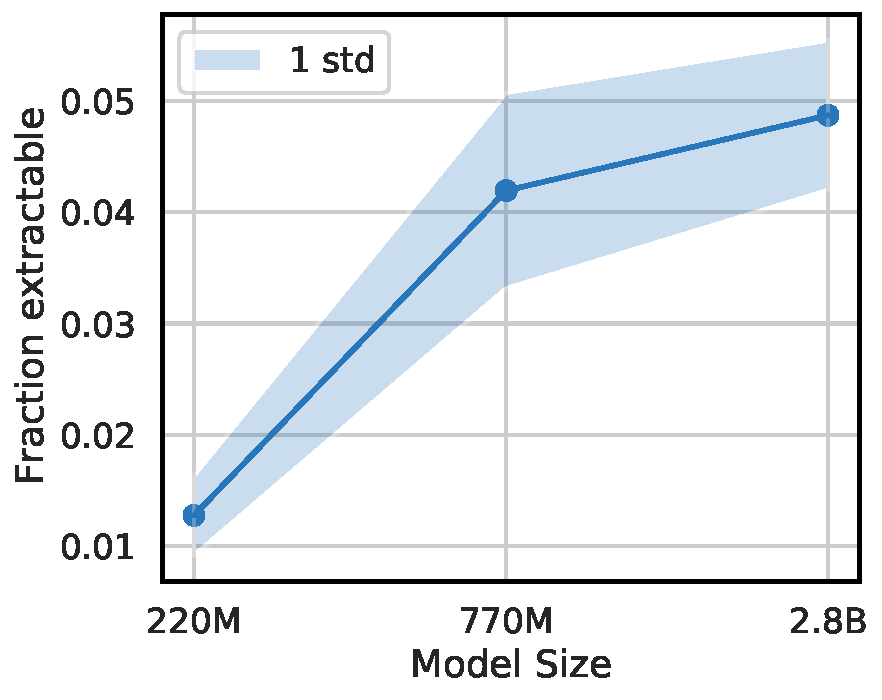
\includegraphics[height=10.5em]{figures/t5_size_vs_extractable_all}
        \caption{}
        \label{fig:other-models-size}
    \end{subfigure}
    \hfill
    \begin{subfigure}[b]{0.32\textwidth}
        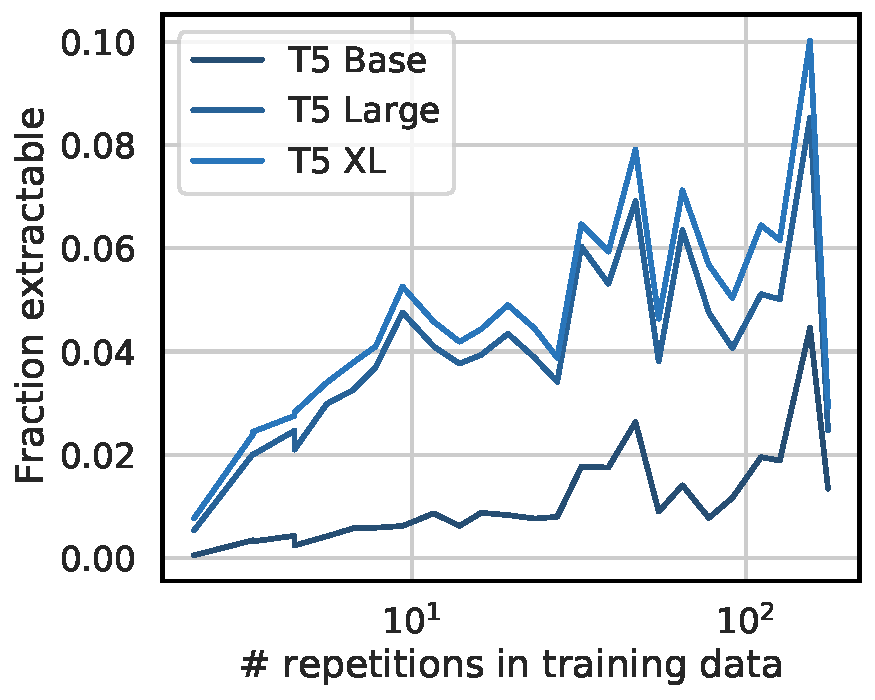
\includegraphics[height=10.5em]{figures/t5_exactly_mem-vs-repetitions-mean-xlabel-ylabel}
        \caption{}
        \label{fig:other-models-dups}
    \end{subfigure}
    \hfill
    \begin{subfigure}[b]{0.32\textwidth}
        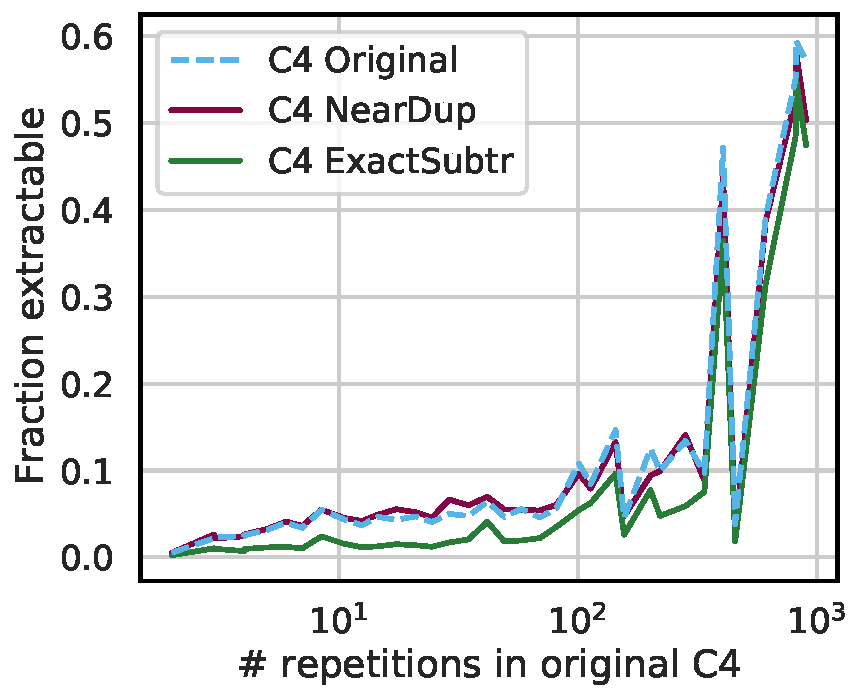
\includegraphics[height=10.5em]{figures/t5dedup_exactly_mem-vs-repetitions-mean}        \caption{}
        % 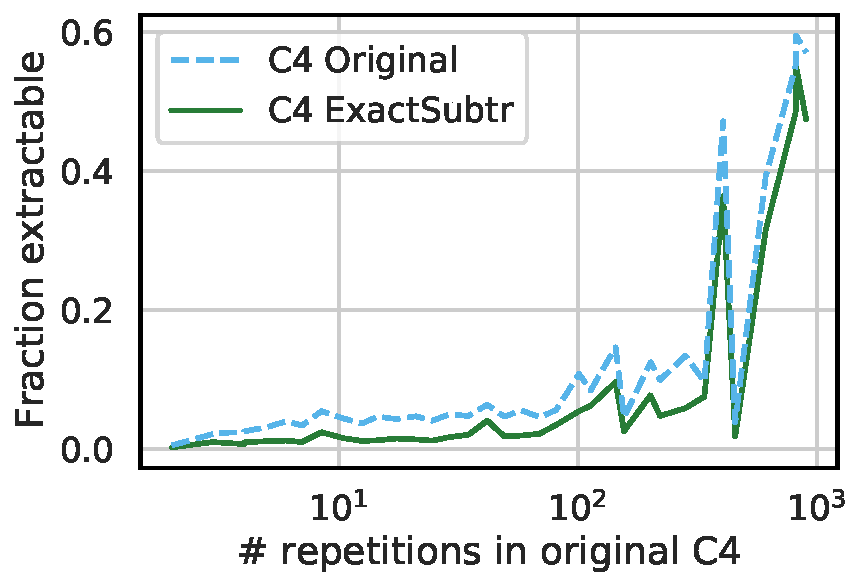
\includegraphics[height=10.5em]{figures/t5dedup_exactly_mem-vs-repetitions-mean_NONEARDUP}
        \label{fig:other-models-dedup}
    \end{subfigure}

    %\begin{overpic}[width=.32\linewidth]{figures/t5_size_vs_extractable_all.pdf}
    %    \put(0,-7){(a)}
    %\end{overpic} 
    %\begin{overpic}[width=.32\linewidth]{figures/t5_exactly_mem-vs-repetitions-mean}
    %    \put(0,-7){(b)}
    %\end{overpic}
    %\begin{overpic}[width=.32\linewidth]{figures/t5dedup_exactly_mem-vs-repetitions-mean}
    %    \put(0,-7){(c)}
    %\end{overpic}
    \vskip-5pt
    \caption{
    \textbf{(a)}
    Masked language model objective: Larger models have a higher fraction of sequences extractable on T5;
    with one standard deviation of variance shaded in dark and the minimum and maximum shaded light.
    \textbf{(b)}
    Masked language model objective: Relationship between number of repetitions and extractable tokens on T5.
    \textbf{(c)}
    Causal language model objective: Relationship between number of repetitions and memorization on language models trained with deduplicated data.
    }
    \label{fig:other-models}
\end{figure*}

The T5 v1.1 models are masked encoder-decoder models trained to reproduce spans that were randomly deleted from an input sequence. The models vary in size from between 77M and 11B billion parameters.
%
These models were trained on C4, a cleaned and filtered version of the English web pages from the Common Crawl, which totals 806 GB in size.
%
At 11 billion parameters, the largest T5 model is the largest publicly available masked language model, making these T5 models a good candidate for studying how memorization scales with model size.

% The first step in this replication study is to 
We must first define what is meant by ``extractable data''
for the masked language modeling task.
T5 models are trained by removing a random $15\%$ of tokens from each training sequence (i.i.d), and the model must then
``fill in the blanks'' to restore the tokens that were dropped from the input.
%
%\todo{random 15\% of tokens that are all over the sequence. Memorized is over a specific masking. }
%
As a result of this different training objective,
Definition~\ref{def:extractable} is not directly applicable because the model does not operate on a \emph{prefix} and output a \emph{suffix}.
We instead define a sequence as memorized if the model \emph{perfectly} solves the masked language modeling task on that sequence.
%
For example, we call a 200-token sequence memorized if the model can
use the 170 ($=200 \cdot 0.85)$) tokens of context to perfectly predict the remaining 30 tokens ($=200 \cdot 0.15$).
%
Because this token-dropping procedure is stochastic, it is possible that one set of dropped tokens might yield
an output of ``memorized'' and another might not.
%
For simplicity, we inspect only one set of masked tokens per sequence; because we are already averaging over
$50,000$ sequences this additional randomness does not harm the results of our analysis.

%
We are able to reproduce the model scaling effect shown in Figure~\ref{fig:main-res-size} for the T5 model family;
Figure~\ref{fig:other-models-size} presents these results.
%
Increasing the number of parameters in the model similarly increases the ability of the model
to perfectly solve the masked prediction task.

Surprisingly, while the overall scaling trend holds true here, we discover an order of magnitude less data in masked models than in a comparably
sized causal language model.
%
For example, the $3$B parameter T5-XL model memorizes just $3.5\%$ of sequences repeated 100 times, compared to the $53.6\%$ of sequences repeated 100 times memorized by GPT-Neo 2.7B (with a context length of 150). 
We believe (without evidence) that this difference can be explained because the choice of tokens to mask at training-time varies for each duplicate of a training example, while causal language models are always provided the same prediction task each time an example and its duplicates are seen during training.

Next, we turn to reproducing the analysis on the effect of duplicate examples in the models' training data on memorization.
%
The situation here becomes significantly less clear.
%
As we can see in Figure~\ref{fig:other-models-dups}, while sequences that have been duplicated more often are easier to memorize,
there is not an obvious log-linear scaling relationship to be found.
%
In particular, compared to the smooth curves we observe in the case of GPT-Neo evaluated on The Pile,
there is significant variance in the results for T5 models trained on C4.
%
Even more surprising is that this variance is \emph{statistically significant}:
sequences repeated between 159 and 196 times are memorized with probability no more than 5.1\% with $99.7\%$ confidence (three standard deviations of variance),
however sequences repeated between 138 and 158 (that is, \emph{less often}) are memorized with probability
at least 6.2\% with $99.7\%$ confidence.
%
That is, for some reason, sequences that occur $\sim$140 times are \emph{more likely to be memorized, despite occurring less often}, even if we assume a three-sigma error in both measurements simultaneously.

In order to explain this counter-intuitive phenomenon, we qualitatively study each of these two buckets
of examples to understand why there is a pronounced difference.
%
Surprisingly, we find that most of the duplicate examples contained in the 138-158 repeat bucket are mostly whitespace tokens, making these sequences much easier to predict correctly than sequences found at other repeat counts.
This effect, to a lesser extent, can be found in other buckets which contain many approximately near duplicates.
%, for example repeatedly listing out various types of birds.

\subsubsection{Language Models Trained on Deduplicated Data}

The models used in \citet{lee2021deduplicating} are 1.5B parameter causal language models.
This model family consists of one model trained on C4 (the same dataset as T5), one model trained on a version of C4 that was deduplicated by removing all documents which were near-duplicates of other documents, and one model trained on a version of C4 that was deduplicated by deleting any string of length-50 tokens that occurred more than once.
\citet{lee2021deduplicating} found that both types of deduplication reduced the likelihood of memorization.

We were most interested in whether models trained on deduplicated data would still exhibit increased memorization of examples which were repeated frequently in the original, non-deduplicated C4 dataset.
% Because \citet{lee2021deduplicating} trained models with few model sizes, we did not perform experiments investigating memorization as a function of scale.
% Because \citet{lee2021deduplicating} only trained models of a fixed size\kl{technically 2 scales}, we are unable to perform experiments that investigate memorization as a function of scale.
%
Figure~\ref{fig:other-models-dedup} plots this fraction of sequences memorized by each of the three models.
%
We draw two interesting conclusions from this data.


First, we find that models trained on deduplicated datasets memorize less data than models trained without deduplicated datasets.
%
For example, for sequences repeated below 35 times, the exact deduplicated model memorizes an average of 1.2\% of sequences, compared to 3.6\% without deduplication, a statistically significant ($p<10^{-15}$) increase by a factor of 3. 
%\todo{the counts used to generate figures are similarly incorrect}
%\todo{include qualitiative examples of the prompts}
Second, while deduplication does help for sequences repeated up to $\sim$100 times,
it does not help for sequences repeated more than this.
%
We observe a spike beginning at 408 repeats: the extractability of the smallest spike is larger than any value before the spike (largest is at 265 repeats, $p<10^{-20}$).
%
We hypothesize that this is due to the fact that any deduplication strategy is necessarily
imperfect in order to efficiently scale to hundreds of gigabytes of training data.
%
% And so while it may be possible for us to remove \emph{most} instances of duplicate data,
% once this data begins to occur thousands of times, the duplicates that slip through
% will result in memorization.
Thus, while it may be possible to remove \emph{most} instances of duplicate data, different and valid definitions of duplicates can mean deduplication is not exhaustive.

\subsection{Conclusion}

%Understanding the degree to which language models memorize their training datasets
%is interesting both to those who care about generalization 
%(because well generalizing models should not focus on the peculiarities of their training dataset), and
%to those who care about privacy (because memorized content can violate the privacy of users in the training dataset).
%
This section presents the first comprehensive quantitative analysis of memorization in
large language models by directly re-processing the training data to identify memorized content.
%
Our work has two broad conclusions.

First, we show that while current LMs do accurately model the distribution of their training data, this does not necessarily imply they will model the desired \emph{underlying} data distribution.
In particular, when the training data distribution is skewed (e.g., by containing many duplicates of some sequences) larger models with more capacity are likely to learn these unintended dataset peculiarities.
%
It therefore becomes even more important to carefully analyze the datasets used to train ever larger models, as future (larger) models are likely to remember even more details than current (smaller) models.


Second, our results indicate that current large language models likely memorize a significant fraction of their training datasets.
%
Memorization scales log-linear with model size---by doubling the number of parameters in a model we can extract a significantly larger fraction of the dataset.
%
Given that current state-of-the-art models contain more than 200$\times$ as many parameters as the largest 6B parameter model we analyze, it is likely that these even larger models memorize many sequences that are repeated just a handful of times.
%
At the same time, we have shown that this memorization is often hard to discover, and for an attack to actually extract this data it will be necessary to develop qualitatively new attack strategies.
%
Fortunately, it appears that (for the comparatively small models we study) training data inserted just once is rarely memorized, and so deduplicating training datasets~\citep{lee2021deduplicating} is likely a practical technique to mitigate the harms of memorization.


\section{Deduplicating Training Data Reduces Memorization}

\subsection{Introduction}
A key factor behind the recent progress in natural language processing is the development of large-scale text corpora used to train increasingly large language models.
These datasets have grown from single gigabytes to as much as a terabyte over the past few years \citep{chelba2013one,xue2020mt5,graff2003english,brown2020language}.
%
Because it is so expensive to perform manual review and curation on massive datasets, they tend to suffer in quality compared to their smaller predecessors.
This has implications far beyond metrics like perplexity and validation loss, as learned models reflect the biases present in their training data \cite{bender2021stochastic,wallace2019universal,sheng2020towards}.
As a result, quantitatively and qualitatively understanding these datasets is therefore a research challenge in its own right \cite{dodge2021documenting}.

%Thus, even though large language models perform well under our current metrics, in large part this is due to the difficulty in creating metrics that adequately capture the nuance in language and human communication \cite{bowman2021fix}.

We show that one particular source of bias,
duplicated training examples, is pervasive:
$10\%$ of the sequences in several common NLP datasets are repeated multiple times.
%Duplicate text in training datasets has four distinct drawbacks.
While naive deduplication is straightforward
(and the datasets we consider already perform some naive form
of deduplication), performing thorough deduplication at scale is both computationally challenging and requires sophisticated techniques.

The simplest technique to find duplicate examples would be to perform exact string matching between all example pairs, but we show this is insufficient since the web containing many docments which are near-duplicates of eacho ther.
This, we introduce two complementary, scalable methods for performing deduplication on documnets which have substantial overlap but may not be identical.
\begin{itemize}
    \item
\textit{Exact} substring matching identifies strings that are repeated verbatim in the train set multiple times.
This allows us to identify cases where only part of a training example is duplicated (\S\ref{sec:exact}).
Using a suffix array \cite{manber1993suffix}, we are able to remove duplicate substrings from the dataset if they occur verbatim in more than one example.
    \item
\textit{Approximate} full document matching uses  MinHash \citep{broder1997resemblance}, an efficient algorithm for estimating the $n$-gram similarity between all pairs of examples in a corpus, to remove entire examples from the dataset if they have high $n$-gram overlap with any other example (\S\ref{sec:approx}).
\end{itemize}

We identify four distinct advantages to training on datasets that have been thoroughly deduplicated.
\begin{enumerate}

\item 
Over $1\%$ of tokens emitted unprompted from a model trained on standard datasets (e.g., C4) are part of a memorized sequence (See \S\ref{sec:memorization-results})---even though the 1.5 billion parameter model is much smaller than the 350GB dataset it was trained on.
By deduplicating the training dataset we reduce the rate of emitting memorized training data by a factor of $10\times$.

\item Train-test overlap is common in non-deduplicated datasets.
For example, we find \emph{a 61-word sequence}%
\footnote{``by combining fantastic ideas, interesting arrangements, and follow the current trends in the field of that make you more inspired and give artistic touches. We'd be honored if you can apply some or all of these design in your wedding. believe me, brilliant ideas would be perfect if it can be applied in real and make the people around you amazed!''} 
in C4 \citep{raffel2019exploring} that is repeated $61{,}036$ times verbatim in the training dataset and $61$ times in the validation set ($0.02\%$ of the samples in each dataset).
This train-test set overlap not only causes researchers to over-estimate model accuracy, but also biases model selection towards models and hyperparameters that intentionally overfit their training datasets.
%Models are therefore \emph{explicitly encouraged} to overfit on the (duplicate) training examples which are likely to appear in the (i.i.d. sampled) validation set as well.
%This overfitting contrasts sharply with how humans learn language \citep{linzen2020can}.

\item Training models on deduplicated datasets is more efficient.
Processing a dataset with our framework requires a CPU-only linear-time algorithm.
And so because 
these datasets are up to $19\%$ smaller, even including the deduplication runtime itself, training on deduplicated datasets directly reduces the training cost in terms of time, dollar, and the environment~\cite{bender2021stochastic, strubell2019energy, patterson2021carbon}.


\item Deduplicating training data does not hurt perplexity: models trained on deduplicated datasets have no worse perplexity compared to baseline models trained on the original datasets. 
In some cases deduplication reduces perplexity by up to $10\%$.
Further, because recent LMs are typically limited to training for just a few epochs \cite{radford2019language,raffel2019exploring},
by training on higher quality data the models can reach higher accuracy faster.
\end{enumerate}
%There is therefore no reason to not perform deduplication, and every reason to perform deduplication.
To summarize, data duplication offers significant advantages and no observed disadvantages.
In the remainder of this section, we present our text deduplication framework and study the extent of duplicate content in common NLP datasets (e.g., C4, Wiki-40B, and LM1B).
We then examine the impact of deduplication on test perplexity and on the frequency of emitting memorized content.
Finally, we analyze to what extent perplexity on existing, released models are skewed as a result of overlap between the train and test/validation splits.

\subsection{Related Work}
\subsubsection{Large Language Model Datasets}
While we believe our results are independent of model architecture,
we perform our analysis on Transformer-based decoder-only language models \citep{vaswani2017attention} trained for open-ended text generation.
These current state-of-the-art models are trained on internet text.
For example, the GPT-2 family of models \citet{radford2019language} is trained on WebText, a dataset of web documents highly ranked on Reddit---however this dataset was not made available publicly.
A common dataset starting point is CommonCrawl, an index of public webpages.
Among the models trained on CommonCrawl include
GPT-3 \cite{brown2020language} with the addition of book datasets,
GROVER \cite{zellers2019defending} on a restricted subset filtered to news domains called RealNews,
and T5 \cite{raffel2019exploring} on a cleaned version of common crawl called C4.
Other models are trained on more curated Internet sources---for example \citet{guo2020wiki40b} used high quality processed Wikipedia text from 40 different languages to train monolingual 141.4M parameter language models.
Non-English models necessarily use different datasets; \citet{zeng2021pangualpha} for instance introduced PANGU-$\alpha$, a family of models with up to 200B parameters that were trained on a non-public corpus of cleaned and filtered Chinese-language documents from CommonCrawl and other sources.
%Lastly, the T5 family of encoder-decoder models was trained on C4, a dataset of cleaned English CommonCrawl documents.
Since many of these datasets are not public,
we deduplicate three that are: Wiki-40B, C4, and RealNews--as well as the One Billion Word Language Model Benchmark \citep{chelba2013one}, 
a smaller
dataset commonly used for evaluation.

Others have observed that popular datasets contain problematic duplicate content.
Bandy et al. \citep{bandy2021addressing} observe that the  Book Corpus \citep{zhu2015aligning}, which was used to train popular models such as BERT, has a substantial amount of exact-duplicate documents according to.
Allamanis et al. \citet{allamanis2019adverse} show that duplicate examples in code datasets cause worsened performance on code understanding tasks.

\subsubsection{Contamination of Downstream Tasks}
When models are trained on datasets constructed by crawling the Internet, it is possible the model will train on the test set of downstream target tasks.
For example, \citet[\S{}4]{radford2019language} performed a post-hoc analysis to identify 8-gram overlaps between GPT-2's training set and datasets used for evaluation,
and \citet{Dodge2021-lb} analyzed C4 and found that up to 14.4\%  of test examples for various standard tasks were found verbatim (normalizing for capitalization and punctuation) in the dataset.
A more proactive approach removes contaminated data.
\citet[Appendix B]{trinh2018simple} removed documents from their CommonCrawl-based train set that overlapped substantially with the commonsense reasoning used for evaluation.
And GPT-3 \cite[\S{}5]{brown2020language} did the reverse and removed downstream evaluation examples from their training data by conservatively filtering out any train set examples with a 13-gram overlap with any evaluation example.
Up to $90\%$ of tasks were flagged as potentially contaminated.
%They found that for some tasks over 90\% of the task examples were flagged as potentially contaminated, but they noted that many detections of contamination were false-positives, and overall the identified contamination did not strongly impact model performance.
% They re-evaluated the models on cleaned datasets, and found that the performance drop was negligible despite heavy (potential) contamination. They hypothesized that either their estimation was too conservative, or that data contamination is no longer an issue in this regime, because the training set is so large that the overfitting of even their largest model (GPT-3 175B) was mild.

In our research, we do not focus on the impact of duplicate text in pretrained models on downstream benchmark tasks; instead we address how duplicate text in the LM training and validation sets impacts model perplexity and the extent to which generated text included memorized content.

\subsubsection{Memorizing training data.} The privacy risks of data memorization, for example the ability to extract sensitive data such as valid phone numbers and IRC usernames, are highlighted by
\citet{carlini2020extracting}.
%
%In this paper we are more interested in the fact that memorization happens, and not the \emph{type} of data being memorized; we treat all instances of the LM generating text that closely matches the training set as problematic.
While their paper finds 604 samples that GPT-2 emitted from its training set, we show that \emph{over $1\%$} of the data most models emit is memorized training data.
% 
In computer vision, memorization of training data has been studied from various angles for both discriminative and generative models~\citep[e.g.][]{arpit2017closer,8953411,feldman2020neural,stephenson2021geometry}
% TODO add citation back in
% teterwak2021understanding}.

\subsection{Datasets Considered}
We analyze the presence of duplicate text in four datasets of varying sizes that have been used for training natural language generation systems, producing general-purpose pre-trained models, and for language model benchmarking.
While this paper restricts itself to English datasets, we expect that non-English datasets suffer from similar issues and could likewise benefit from de-duplication.

\subsubsection{Wikipedia (Wiki-40B)}
consists of multi-lingual cleaned Wikipedia text \citep{guo2020wiki40b}.
We take the English portion, which contains 2.9M Wikipedia pages with an average length of 768 BPE tokens.
The dataset creators do not indicate any deduplication was performed aside from removing redirect-pages (e.g., ``sunflower'' to ``Helianthus'').

\subsubsection{One-Billion Word benchmark (LM1B)}  contains 30M sentences of news commentary \citep{chelba2013one}.
Unlike the other datasets we analyze, LM1B's examples are one sentence long rather than multi-sentence documents.
The average example length is 32 BPE tokens.
While this dataset is extremely standard for benchmarking language models, \citet[Sec 4]{radford2019language} note it has 13.2\% overlap of the test set with the train set.

\subsubsection{Colossal Cleaned Common Crawl (C4)}
is made up of 360M web documents, with an average length of 486 BPE tokens \citep{raffel2019exploring}.
C4 was introduced as a pre-training dataset for T5, a set of encoder-decoder models which have been widely used in fine-tuned downstream tasks.
The dataset was previously deduplicated in a more sophisticated process
than the prior two datasets.
Each paragraph was hashed and paragraphs resulting in hash collisions were removed.
This was followed by a pass that removed placeholder text, code, and prohibited words.
See \citet{dodge2021documenting} for a detailed breakdown of the source text in C4.


\subsubsection{RealNews}
is a subset of the Common Crawl consisting of articles from news domains \citep{zellers2019defending}.
%RealNews was used as the training data for GROVER, a controllable language model designed to generate news articles given metadata such as the article's publisher or title.
It contains 31M documents with average length 793 BPE tokens.
RealNews was deduplicated by inserting a hash of the first 100 characters of each document into a bloom filter \citep{bloom1970space} and then excluding any document which resulted in a hash collision.
% an one already added to the dataset. TODO add back in
Like C4, examples with duplicate URLs were excluded.


% In all the datasets studied here, an example corresponds to a \emph{document}, except for LM1B, in which an example corresponds to a \emph{sentence}.
\subsection{Method for Exact Substring Duplication} \label{sec:exact}
We consider a dataset $D = \{x_i\}_{i=1}^N$ as a collection of \emph{examples} $x_i$.
Each of these examples is itself a sequence of \emph{tokens}: $x_i = \left[ x_i^1, x_i^2, \cdots, x_i^{s_i} \right]$.

Due to the diversity of possibilities in human language, it is rare for the same idea to be expressed identically in multiple documents unless one expression is derived from the other, or both are quoting from a shared source.
This observation motivates deduplicating exact substrings. We call our approach \Exact{}.
When two examples $x_i$ and $x_j$ share a sufficiently long substring (that is, a substring for which $x_i^{a..a+k} = x_j^{b..b+k}$), that substring is removed from one of them.

\subsubsection{Suffix Arrays}
This exact-substring-matching criterion, while conceptually simple, is computationally prohibitive with naive (quadratic) all-pair matching.
%
To improve the efficiency, we concatenate all the examples of the entire dataset $D$ into a giant sequence $\mathcal{S}$, and construct a Suffix Array $\mathcal{A}$ of $\mathcal{S}$.
A suffix array \citep{manber1993suffix} is a representation of a suffix tree \citep{weiner1973linear} that can be constructed in linear time in $\lVert \mathcal{S} \rVert$ \citep{karkkainen2003simple}  
and enables efficient computation of many substring queries; in particular, they allow us to identify duplicated training examples in linear time.
Suffix arrays have the advantage over suffix trees in that they are 10--100$\times$
more memory efficient \cite{manber1993suffix}, requiring just 8 bytes per input token, though they are asymptotically less
efficient for some query types.
They have been used widely in NLP, such as for efficient TF-IDF computation \citep{yamamoto2001using} and document clustering \citep{hung2007new}.


The suffix array $\mathcal{A}$ for a sequence $\mathcal{S}$ is a lexicographically-ordered list of all suffixes contained in the sequence. 
%
%That is, formally, the suffix array is defined by the computation
Formally,
\[ \mathcal{A}(\mathcal{S}) = \mathop{\text{arg sort}} \text{all\_suffixes}(\mathcal{S}) \]
%
For example, the suffixes of the sequence ``banana'' are (``banana'',  ``anana'', ``nana'' ``ana'', ``na'', ``a'')
and so the suffix array is the sequence (6 4 2 1 5 3).
In practice, we construct $\mathcal{S}$ from the BPE tokenization of the text (\S\ref{sec:impact-trained-models}).

% Suffix arrays are often preferable to suffix trees because, while asymptotically less
% efficient for some types of queries, they are 10-100$\times$
% more memory efficient \cite{manber1993suffix}, requiring just 8 bytes per input token.

%% TODO FIGURE 1 GOES HERE


\subsubsection{Substring matching}

After constructing $\mathcal{A}$, it is straightforward to identify duplicated training examples.
Suppose that the sequence $s$ was repeated exactly twice in the training dataset $\mathcal{S}$ at positions $i$ and $j$,
that is, $\mathcal{S}_{i..i+|s|} = \mathcal{S}_{j..j+|s|}$.
%
Then the indices $i, j$ will occur adjacent to each other in the suffix array $\mathcal{A}$.

Finding all repeated sequences is thus a matter of linearly scanning the suffix array from
beginning to end and looking for sequences $\mathcal{A}_i, \mathcal{A}_{i+1}$ that share a common prefix of
at least some threshold length.
%
Any satisfying sequences are recorded.
%

\subsubsection{Setting a Threshold of Duplicates}
\label{section:exact_thresh}
One important question is how long a substring match must be before we ought to count it as a duplicate.
%
In Figure~\ref{fig:suffix-match-len}, we plot the frequency of substring matches within the four datasets we will
consider.
For each substring of length $k$, we compute the probability that there exists another sequence of length $k$ identical to this one; formally:
\[m(k) = \mathop{\text{Pr}}_{i \in [N]}\big[ \exists j \ne i : \mathcal{S}_{i..i+k} = \mathcal{S}_{j..j+k}\big].\]
We choose $50$ tokens as the threshold to be conservative:
the ``bend in the knee'' occurs at $10$ tokens, and manual inspection of
length-$25$ matches found no false positives.
We then doubled this value to have an exceptionally large margin for error.

\begin{figure}
    \centering
    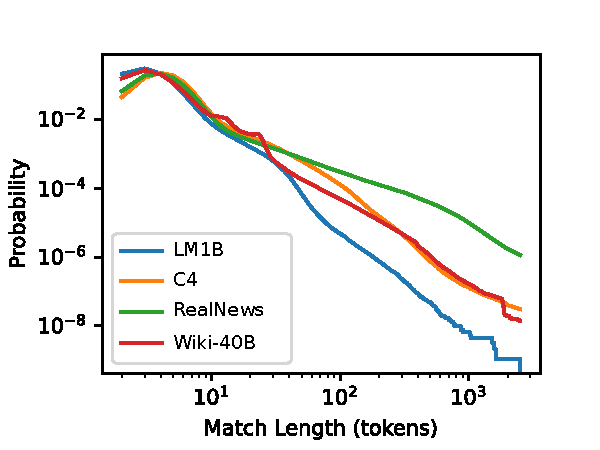
\includegraphics[scale=.8]{figures/match_length.pdf}
    \caption{For each substring of length $k$,
    we plot the probability that there exists a second identical length-$k$ substring in the same train set.
    Matches with length under $10$ subword tokens are common, and account for $90\%$ of tokens.
    We choose a threshold of 50 for experiments.
    % For future experiments, we use $50$ tokens as the threshold for memorization.
    }
    \label{fig:suffix-match-len}
\end{figure}


\subsubsection{Implementation}
\paragraph{Parallel linear time construction.}
We build a parallelized linear time suffix array algorithm.
%
As a building block, we make black-box use of the SA-IS algorithm for
constructing a suffix array in linear time \citet{nong2009linear,ko2003space}.
%
Unfortunately, this algorithm is not easily parallelized directly, so
we introduce a simple divide and conquer approach to parallelizing the array construction.


We build our implementation in Rust and extend an existing suffix array library\footnote{https://github.com/BurntSushi/suffix}
with three modification.
The first two are straightforward implementation differences:
we modify the code to allow datasets larger than $4$GB,
and we remove the requirement that strings parse as valid UTF-8 sequences in favor of raw byte sequences.
Our third change is more significant: we re-implement the algorithm
so that we can stream the suffix array itself off disk.

\paragraph{Parallel partial suffix array construction.}
%
Our divide and conquer suffix array construction algorithm starts by 
partitioning the dataset into $K$ different ``splits'' with SA-IS run
over independently on each split in parallel.
%
This algorithm still requires $O(N)$ work but runs in $O(N/K)$ wall-clock time.
%
This gives us $N$ separate suffix arrays $\mathcal{A}^i$.

Given two suffix arrays $A_1$ and $A_2$ for two sequences $S_1$ and $S_2$ it's not completely trivial to construct a single suffix array $A$ for $S = S_1 \mid\mid S_2$ 
because of the boundary conditions.
Instead, we don't build the data $S = S_1 \mid\mid S_2$ but rather let $S_1' = S_1 \mid\mid S_2[upto K]$ for some $K$ greater than the longest substring match.
Then we build the arrays on $S'_1$ and $S_2$.
To merge the arrays together we can remove the items from the first array after index $|S_1|$ and merge-sort insert them into the second.

\paragraph{Parallel merge of partial suffix arrays.}
We now merge these separate arrays together into a single suffix array $\mathcal{A}$,
%
Consider the simpler case of two partial suffix arrays $B$ and $C$ that we 
would like to merge together.
%
We can achieve this by letting $i=0$ index $B$ and $j=0$ index $C$.
%
Each iteration of the algorithm then pushes $B_i$ into $\mathcal{A}$ if
$S_{B_i..} < S_{C_i}$ and $C_i$ otherwise, repeating until $i=|B|-1$ and $j=|C|-1$.
%
To generalize to $K$ splits, we need only replace the single comparison above with
a min-heap requiring $O(\log{K}) \ll 10$ work on each iteration.

Observe that in the general case this algorithm is $O(N m \log(K))$ where $N$ is the length
of the dataset, $m$ is the average length of a prefix match, and $K$ is the number of splits.
%
It is therefore incorrect to call this algorithm linear time in the general case, for ours it is.
%
Because the length of the longest match is bounded above by the length of the longest
sequence, as long as the size of the dataset is independent of the length of the 
longest sequence in the dataset, this algorithm remains efficient.

Again, we can parallelize this operation among $L$ simultaneous jobs 
(in practice we set $K=L$ as the number of threads on our machine).
%
In the $K=2$ case, job $l$ processes $i \in [jN/L, (j+1)N/L]$, choosing
the bounds of $j$ by binary searching into $C$ so that $S_{B_{i}} < S_{C_{j}} < S_{B_{j+1}}$.
%
The case where $K>2$ is identical except that we repeat this over all $K$ partial suffix arrays.


\subsubsection{Computational Analysis}
We run our algorithm on a single VM on the cloud with $96$ cores and $768$GB of memory.
Our algorithm is efficient, for example processing the Wiki-40B training set ($3$ million
examples containing $4$GB of text) in $2.3$ minutes wall-clock time ($2.1$ CPU-hours of work).
%
The $350$GB C4 dataset takes under 12 hours (wall-clock) to build a suffix array; although we are still memory constrained and so this corresponds to $\sim 1000$ CPU-hours. 
% 
Once the suffix array has been constructed, it takes under an hour to deduplicate the C4 dataset.


Note that this algorithm still requires that the dataset itself fits in memory
(so that we can efficiently index in arbitrary positions), but we do not need to fit the entire suffix array into memory.
This is fortunate since our suffix array requires an $8\times$ space overhead.
For example, the suffix array for the
$350$GB C4 is $1.5$TB.

%

Compared to the cost of training a language model on this dataset, the additional
work required to deduplicate the training dataset is negligible.





%%%%%%%%%%%%%%%%%%%%%%%%%

% % Table generated by Excel2LaTeX from sheet 'Sheet3'
% \begin{table*}[htbp]
%   \small
%   \centering
%     \begin{tabular}{l|p{0.45\linewidth}|p{0.45\linewidth}}
%     \toprule
%     \multicolumn{1}{c|}{Dataset} & \multicolumn{1}{c|}{Example} & \multicolumn{1}{c}{Near-Duplicate Example} \\
%     \hline
%     Wiki-40B & \textbackslash{}n\_START\_ARTICLE\_\textbackslash{}nHum Award for \hl{Most Impactful Character}\textbackslash{}n\_START\_SECTION\_\textbackslash{}nWinners and nominees\textbackslash{}n\_START\_PARAGRAPH\_\textbackslash{}nIn the list below, winners are listed first in the colored row, followed by the other nominees. [...] & \textbackslash{}n\_START\_ARTICLE\_\textbackslash{}nHum Award for \hl{Best Actor in a Negative Role}\textbackslash{}n\_START\_SECTION\_\textbackslash{}nWinners and nominees\textbackslash{}n\_START\_PARAGRAPH\_\textbackslash{}nIn the list below, winners are listed first in the colored row, followed by the other nominees. [...] \\
%     \hline
%     LM1B  & I left for California in 1979 and tracked Cleveland 's changes on trips back to visit my sisters . & I left for California in 1979 \hl{,} and tracked Cleveland 's changes on trips back to visit my sisters . \\
%     \hline
%     RealNews & KUALA LUMPUR (Reuters) - Roads in Southeast Asia have been getting a little louder lately as motorcycle makers, an aspiring middle class and easy bank credit come together to breed a new genus of motorcyclists -- the big-bike rider. [...] & \hl{A visitor looks at a Triumph motorcycle on display at the Indonesian International Motor Show in Jakarta September 19, 2014. REUTERS/Darren Whiteside\textbackslash{}n}KUALA LUMPUR (Reuters) - Roads in Southeast Asia have been getting a little
%     % louder lately as motorcycle makers, an aspiring middle class and easy bank credit come together to breed a new genus of motorcyclists -- the big-bike rider.
%     [...] \\
%     \hline
%     C4    & Affordable and convenient holiday flights take off from your departure country, \hl{"Canada"}. From \hl{May 2019} to October 2019, Condor flights to your dream destination will be roughly \hl{6} a week! Book your \hl{Halifax (YHZ) - Basel (BSL)} flight now, and look forward to your \hl{"Switzerland"} destination! & Affordable and convenient holiday flights take off from your departure country, \hl{"USA"}. From \hl{April 2019} to October 2019, Condor flights to your dream destination will be roughly \hl{7} a week! Book your \hl{Maui Kahului (OGG) - Dubrovnik (DBV)} flight now, and look forward to your \hl{"Croatia"} destination!" \\
%     \bottomrule
%     \end{tabular}%
%   \caption{Qualitative examples of new-duplicate examples identified by \Approx{} from each dataset. Notable differences have been highlighted.}
%   \label{tab:qualitative_examples}%
% \end{table*}%

% Table generated by Excel2LaTeX from sheet 'Sheet3'
\begin{table*}[htbp]
  \caption{Qualitative examples of near-duplicates identified by \Approx{} from each dataset. The similarity between documents is highlighted. Note the small interspersed differences that make exact duplicate matching less effective. Examples ending with ``[...]'' have been truncated for brevity.
  More data available in Appendix.}
  \label{tab:qualitative_examples}%
  \scriptsize
  \centering
    \begin{tabular}{l|p{0.39\linewidth}|p{0.41\linewidth}}
    \toprule
    \multicolumn{1}{c|}{Dataset} & \multicolumn{1}{c|}{Example} & \multicolumn{1}{c}{Near-Duplicate Example} \\
    \midrule
    Wiki-40B & \pl{\textbackslash{}n\_START\_ARTICLE\_\textbackslash{}nHum Award for } {Most Impactful Character} \pl{\textbackslash{}n\_START\_SECTION\_\textbackslash{}nWinners and nominees\textbackslash{}n\_START\_PARAGRAPH\_\textbackslash{}nIn the list below, winners are listed first in the colored row, followed by the other nominees.} [...] &
    \pl{\textbackslash{}n\_START\_ARTICLE\_\textbackslash{}nHum Award for} {Best Actor in a Negative Role} \pl{\textbackslash{}n\_START\_SECTION\_\textbackslash{}nWinners and nominees\textbackslash{}n\_START\_PARAGRAPH\_\textbackslash{}nIn the list below, winners are listed first in the colored row, followed by the other nominees.} [...] \\
    \midrule
    LM1B  & \pl{I left for California in 1979 and tracked Cleveland 's changes on trips back to visit my sisters .} & \pl{I left for California in 1979} , \pl{and tracked Cleveland 's changes on trips back to visit my sisters .} \\
    %\midrule
    %RealNews & \pl{KUALA LUMPUR (Reuters) - Roads in Southeast Asia have been getting a little louder lately as motorcycle makers, an aspiring middle class and easy bank credit come together to breed a new genus of motorcyclists -- the big-bike rider.} [...] &
    %{A visitor looks at a Triumph motorcycle on display at the Indonesian International Motor Show in Jakarta September 19, 2014. REUTERS/Darren Whiteside\textbackslash{}n} \pl{KUALA LUMPUR (Reuters) - Roads in Southeast Asia have been getting a little [...] big-bike rider.} [...]
    % louder lately as motorcycle makers, an aspiring middle class and easy bank credit come together to breed a new genus of motorcyclists -- the big-bike rider.
    %\\
    \midrule
    C4    & \pl{Affordable and convenient holiday flights take off from your departure country,} "Canada"\pl{. From} May \pl{2019 to October 2019, Condor flights to your dream destination will be roughly} 6 \pl{a week! Book your} Halifax (YHZ) - Basel (BSL) \pl{flight now, and look forward to your} "Switzerland" \pl{destination!} &
    \pl{Affordable and convenient holiday flights take off from your departure country,} "USA"\pl{. From} April \pl{2019 to October 2019, Condor flights to your dream destination will be roughly} 7 \pl{a week! Book your} Maui Kahului (OGG) - Dubrovnik (DBV) \pl{flight now, and look forward to your} "Croatia" \pl{destination!} \\
    \bottomrule
    \end{tabular}%
\end{table*}%




\subsection{Method for Approximate Matching with MinHash} \label{sec:approx}

\subsubsection{Overview}

We also perform \emph{approximate} deduplication based on matching entire examples.
This method, which we call \Approx, is a good complement to the \emph{exact} substring matching, especially for web crawl text, as it handles the very common case of documents being identical except for interspersed templated fields (such as the last row of Table \ref{tab:qualitative_examples}).

MinHash \citep{broder1997resemblance} is an approximate matching algorithm widely used in large-scale deduplication tasks \citep{versley2012not,GABRIEL201863,gyawali2020deduplication}, including to deduplicate the training set for a large Chinese-language LM \citep{zeng2021pangualpha}.
Given two documents $x_i$ and $x_j$, the main idea is to represent each document by its respective set of $n$-grams $d_i$ and $d_j$.
We can then use hash functions to approximate the \emph{Jaccard Index} \citep{jaccard1912distribution}:
\begin{equation}
% \operatorname{Jaccard}(d_i, d_j) = s_{i, j} := \frac{|d_i \cap d_j|}{|d_i \cup d_j|}
%\operatorname{Jaccard}(d_i, d_j) = \frac{|d_i \cap d_j|}{|d_i \cup d_j|}
\operatorname{Jaccard}(d_i, d_j) = \nicefrac{|d_i \cap d_j|}{|d_i \cup d_j|}
\end{equation}
If the Jaccard Index between $d_i$ and $d_j$ is sufficiently high, it is likely that documents are approximate matches of each other.
To efficiently approximate the Jaccard index, MinHash constructs document signatures by sorting each of the $n$-grams via a hash function, and then keeping only the $k$ smallest hashed $n$-grams.
There are multiple ways to construct estimators of the Jaccard index from these kinds of signatures \citep{cohen2016min}.

In our implementation, we use 5-grams and a signature of size 9,000. The probability that two documents are considered a potential match is
\begin{equation}
\operatorname{Pr}(d_i, d_j | \operatorname{Jaccard}(d_i, d_j) = s_{i, j}) = 1 - (1 - s_{i, j}^b)^r
\end{equation}
where $b=20$ and $r=450$ are user-settable parameters to control the strength of the filter.

For each pair of documents identified as a potential match, more computationally expensive similarity metrics can be employed as a subsequent filtering step.
In particular, we identify two documents as duplicates if they are matched by the MinHash algorithm and their \emph{edit similarity} is greater than 0.8. The edit similarity between token sequences $x_i$ and $x_j$ is defined as:
\begin{equation}
    \operatorname{EditSim}(x_i, x_j) = 1 - \frac{\operatorname{EditDistance}(x_i, x_j)}{\max(|x_i|, |x_j|)}
\end{equation}

\noindent To build clusters of similar documents, we construct a graph that has an edge between two documents if they are considered a match. Then, we use the method introduced in \citet{lacki2018connected} to identify  connected components.
%

\subsubsection{Implementation Details}
\label{section:minhash_details}
For our MinHash based deduplication method, documents are first space tokenized, then each consecutive 5-gram is hashed using tabulation hashing.
The set of these hashes is the signature for the document.
For each element in a document's signature, the element is hashed using $k$ other hash functions.
The minimum hashed element for each of the $k$ hash functions is stored.
These minimum hashes are then partitioned into $r$ buckets, with $b$ hashes per bucket.
These $b$ hashes are augmented into a single value, then if two documents have the same value in at least one bucket, they'll be marked as a potential match.
The probability that two documents are considered a potential match is equal to
\begin{equation}
\operatorname{Pr}(d_i, d_j | \operatorname{Jaccard}(d_i, d_j) = s_{i, j}) = 1 - (1 - s_{i, j}^b)^r
\end{equation}
where $s_{i,j}$ is the Jaccard index between the two documents.
For document pairs that were identified as potential matches, we computed their actual Jaccard index, and if that was above 0.8, we computed their edit similarity.
Document pairs with edit similarity higher than 0.8 were identified as duplicates.
After some experimentation, we chose to use $b=20$, and $r=450$, so $k=9,000$, so as to make sure a collision at the desired Jaccard index threshold of 0.8 had a high probability of occurring
% $k=9,000$, $b=20$, and $r=450.
% $k=800$, $b=20$, and $r=40$.

\subsubsection{Computational Analysis}
% Our Minhash algorithm works by generating $B$ hash signatures for each document, grouping the documents by each signature to form buckets, randomly sampling $K$ documents within each bucket. Pairwise comparisons are made between the elements within each sample.

Let $N$ be the number of documents and $T$ be the maximal number of tokens in a document. Edit similarity has a worst case complexity of $T^2$, so the worst case complexity is

\begin{equation}
    O(N + b k^{2} T^{2} N) = O(N)
\end{equation}

\noindent since $b$, $k$, and $T$ are all $\ll$ $N$. The left term is the complexity of grouping by the signatures, and the right represents the pathological worst case of all documents falling into the same $B$ buckets.

The highly distributed \Approx{} implementation we employed is one used for large-scale production tasks at Google.
On the English C4 dataset, the algorithm consumed approximately 41.5 kWh of energy.
Note that our choices of $k$ and $b$ were designed to produce very high recall, and with different parameters, the algorithm could be made much more energy efficient while producing similar results.


\begin{figure}[t]
    \centering
    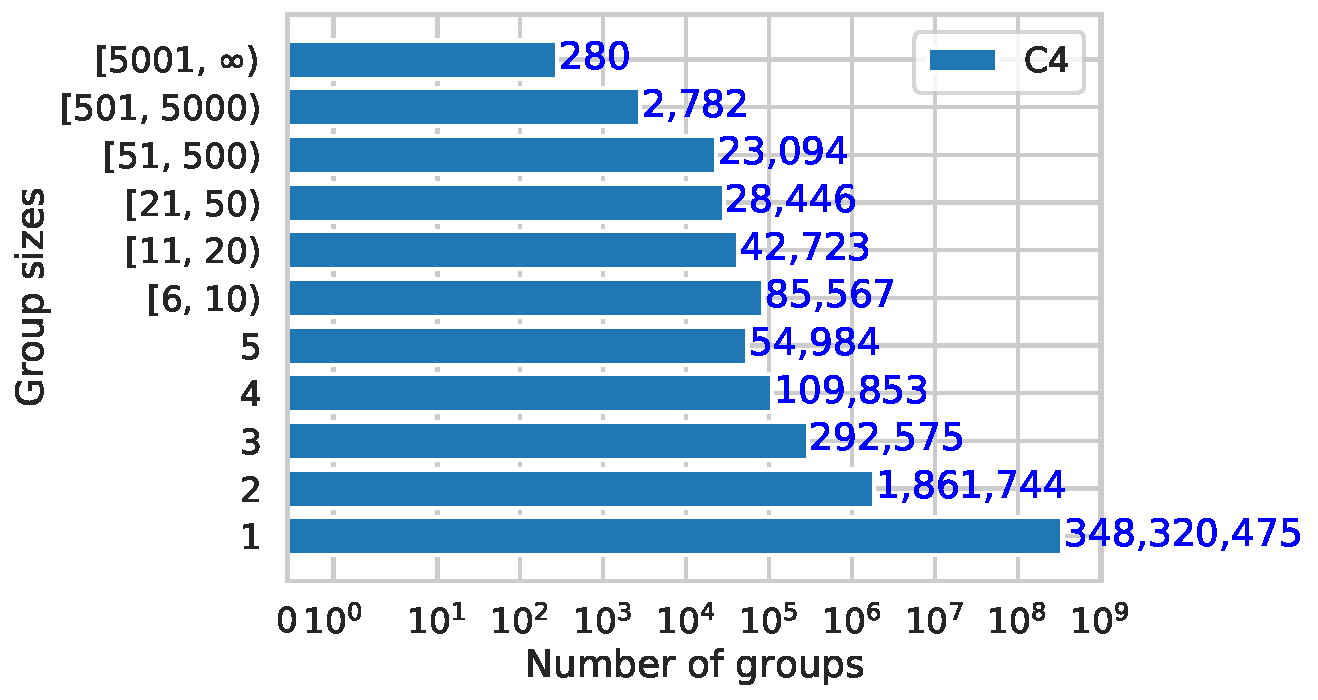
\includegraphics[width=0.6\linewidth]{figures/nd3/nd3-cluster-hist-c4.pdf}
    \caption{The distribution of near-duplicate cluster sizes from running \Approx{} on C4.}
    \label{fig:nd3-cluster-hist-c4}
\end{figure}

\subsection{Results}\label{sec:deduplication-results}
We deduplicate each of the four datasets with both of our two techniques.
When text was duplicated across multiple data splits, we prioritized keeping a copy in the test or validation set and removing it from the train set.
%, so we can have comparable evaluation sets.
%
% For each dataset, we measure several properties.

% Other examples from the same split that are duplicate (e.g., irrelevant training examples).




\subsubsection{Amount of Text Removed}
% We find that existing text datasets scraped from the internet contain duplicated content.
% While both C4 and RealNews explicitly attempt to perform deduplication [cites], they only deduplicate \emph{exact matches} of entire training sequences. 
% This underestimates the amount of duplications in the dataset. 
With \Approx{}, we found that the web-scrape datasets contain between 3.04\% (on C4) to 13.63\% (on RealNews) near duplicates (Table \ref{tab:num_duplicates}).
Near-duplicate text is much less common in Wiki-40B, forming only 0.39\% of the train set.\footnote{Most duplicates we saw were automatically generated pages, such as the outcomes of sports games.
This shows the strength of manual curation for creating high-quality datasets.}
In C4, the majority (1.8M) of near-duplicate clusters consisted of just a single pair of examples that matched against each other, but there were 280 clusters with over 5,000 examples in them (Figure \ref{fig:nd3-cluster-hist-c4}), including one cluster of size 250,933.

On average with \Exact{}, we remove more total content than with \Approx{} (despite \Exact{} not removing any examples outright)---for example removing $7.18\%$ of the tokens in C4.
%
The exception is LM1B, where \Exact{} removes $8\times$ less data than
\Approx{}.
On investigation, we find this is due to the fact that LM1B documents are significantly shorter: $90\%$ of all documents are under 50 tokens, and so are not even candidates for potential matches even if the entire sequence matched verbatim.
%
We find that both \Approx{} and \Exact{} remove similar content---$77\%$ of the training examples that \Approx{} removes from C4 have at least one verbatim length-$50$ match found by \Exact{}.




% Edit this: https://docs.google.com/spreadsheets/d/1VDy_TtaEN8eO9Aj5OYso-txrz4BRrV_IXOLE1YwWKAE/edit?resourcekey=0-4uqN2Jj_pYKxxAwORZUScA#gid=0
% \begin{table*}[]
% \centering 
% \small
% \begin{tabular}{l|rrrrrrrl}
% \toprule
% Dataset & \multicolumn{1}{l}{\# Train Ex} & \multicolumn{2}{l}{\# Duplicates in Train} & \multicolumn{2}{l}{Most Duplicate} & \multicolumn{1}{l}{\# Test Ex} & \multicolumn{2}{l}{\# Test Ex in Train} \\
%  & \multicolumn{1}{l}{} & \multicolumn{1}{l}{\Approx} & \multicolumn{1}{l}{\Exact} & \Approx & \multicolumn{1}{r}{\Exact} & \multicolumn{1}{l}{} & \multicolumn{1}{l}{\Approx} & \Exact \\
% \midrule
% C4 & 364,865,800 & 11,077,485 & 63,396,191 & 250,933 & 224,323 & 364,608 & 16,756 &  \\
% Real News & 31,158,659 & 4,247,409 & 10,567,686 & 3,002 & 131,853 & 1,639,104 & 235,235 &  \\
% LM1B & 30,301,028 & 1,474,048 & 105,906 & 143 & 4,154 & 306,688 & 15,083 &  \\
% Wiki40B & 2,926,536 & 11,487 & 283,667 & 855 & 1,121 & 162,274 & 1,163 & \\
% \bottomrule
% \end{tabular}

% \caption{On the left, the total number of examples in the train set for each dataset, and the number of examples that were identified as containing duplicate text.
% On the right, the total number of examples in the validation set for each dataset, and the fraction of validation set examples which contained duplicate text with the train set.}
% \label{tab:num_duplicates}
% \end{table*}
    
\begin{table}[tbp]
  \centering
  \small
    \begin{tabular}{l|rr|r}
    \toprule
          & \multicolumn{2}{c}{\% train examples with} & \multicolumn{1}{c}{\% valid with} \\
          & \multicolumn{1}{c}{dup in train} & \multicolumn{1}{c}{dup in valid} & \multicolumn{1}{c}{dup in train} \\
          \midrule
    C4    & 3.04\% & 1.59\% & 4.60\%  \\
    RealNews & 13.63\% & 1.25\% & 14.35\%  \\
    LM1B  & 4.86\% & 0.07\% & 4.92\%  \\
    Wiki40B & 0.39\% & 0.26\% & 0.72\% \\
    \bottomrule
    \end{tabular}%
  \caption{The fraction of examples identified by \Approx{} as near-duplicates.}
  \label{tab:num_duplicates}%
\end{table}%

\begin{table}[tbp]
  \centering
  \small
    \begin{tabular}{l|S[table-format=3.2]S[table-format=3.3]|S[table-format=3.3]}
    \toprule
          & \multicolumn{2}{c}{\% train tokens with} & \multicolumn{1}{c}{\% valid with} \\
          & \multicolumn{1}{c}{dup in train} & \multicolumn{1}{c}{dup in valid} & \multicolumn{1}{c}{dup in train} \\
          \midrule
    C4    & 7.18\% & 0.75\%  & 1.38\% \\
    RealNews & 19.4\%  & 2.61\%  & 3.37\% \\
    LM1B  & 0.76\%  & 0.016\%  & 0.019\% \\
    Wiki40B & 2.76\%  & 0.52\%  & 0.67\% \\
    \bottomrule
    \end{tabular}%
  \caption{The fraction of tokens  (note Table~\ref{tab:num_duplicates} reports the fraction of \emph{examples}) identified by \Exact{} as part of an exact duplicate 50-token substring.}
  \label{tab:num_duplicates2}%
\end{table}%
\begin{table*}[ttbp]
  \caption{On the left, we show the URLs that had the greatest proportion of examples marked as near-duplicates by \Approx (filtered to URLs which occurred at least 10 times). On the right, we show the 20 most frequent URLs in C4 for which all examples were marked as near-duplicates by \Approx.}
  \label{tab:urls}%
  \centering
  \small
    \begin{tabular}{lrr||lrr}
    \toprule
    \multicolumn{1}{c}{RealNews Url} & \multicolumn{1}{c}{\# Total} & \multicolumn{1}{c}{Frac Dups} & \multicolumn{1}{c}{C4 Url} & \multicolumn{1}{c}{\# Total} & \multicolumn{1}{c}{Frac Dups} \\
    \hline
    medicalnewstoday.com. & 12    & 1.00  & hairtechkearney.com & 4883  & 1 \\
    dodbuzz.com & 301   & 0.99  & keywordsking.com & 1786  & 1 \\
    undertheradar.military.com & 187   & 0.97  & sydneysitalianfruitshops.online & 1178  & 1 \\
    q.usatoday.com & 33    & 0.94  & moewiki.usamimi.info & 1001  & 1 \\
    ad-test.thirdage.com & 354   & 0.94  & swarovskijewelryoutlet.org & 984   & 1 \\
    amp.nymag.com & 15    & 0.93  & forzadurto.org & 980   & 1 \\
    citizenwire.com & 1022  & 0.93  & producerati.com & 971   & 1 \\
    paycheck-chronicles.military.com & 363   & 0.92  & sourceryforge.org & 908   & 1 \\
    product-reviews.net & 73403 & 0.92  & heavenz-kitchen.com & 876   & 1 \\
    kitup.military.com & 196   & 0.92  & little-eclipse.com & 822   & 1 \\
    gcaptain.com & 33903 & 0.92  & walops.com & 819   & 1 \\
    dev.screenrant.com & 70    & 0.91  & 16thstlaunderland.com & 713   & 1 \\
    live.swissinfo.ch & 66    & 0.91  & theroyalstarinfo.com & 696   & 1 \\
    news.theepochtimes.com & 82    & 0.87  & code4kt.com & 684   & 1 \\
    opinion.toledoblade.com & 986   & 0.87  & nflfalconsjerseys.us & 682   & 1 \\
    cdn.moneytalksnews.com & 121   & 0.86  & quiltingbeeshop.com & 676   & 1 \\
    amp.fox23.com & 14    & 0.86  & ulifeinsurancemiami.com & 675   & 1 \\
    sales.rollingstone.com & 20    & 0.85  & wowkeyword.com & 673   & 1 \\
    ftp.screenrant.com & 20    & 0.85  & taspetro.com & 671   & 1 \\
    \bottomrule
    \end{tabular}%
\end{table*}%

\subsection{Properties of Duplicated Text}
While the authors of both RealNews and C4 explicitly attempted deduplication during dataset construction, the methods were insufficient to capture the more subtle types of duplicate text commonly found on the internet.
In C4 and Wiki-40B, we qualitatively observe that much of the text identified as near-duplicated is computer-generated.
The text is identical except for the names of places, businesses, products, dates, and so on. 
Because these examples frequently differ by just a few words at a time, deduplication strategies relying on exact string matching would fail to identify a match.
Example duplicate pairs from each dataset can be found in Table \ref{tab:qualitative_examples}.
Table \ref{tab:urls} shows the URLs had the largest proportion of examples identified by \Approx{} as near-duplicates. 
For C4, these tend to be websites that sell many similar products and thus have a large amount of templated text.
For RealNews, content aggregators seem especially common.

For RealNews and LM1B, derived from news sites, we observe that many near-duplicates occur because the same news article appears on multiple news sites with slightly different formatting.
For example, in LM1B, there is one example that starts ``\textit{MINEOLA , N.Y. - New York officials say} [...]'' and another that starts ``\textit{( AP ) - New York officials say} [...]''.
The two examples are otherwise identical.

\subsubsection{Train / Test Set Leakage}
\label{sec:leakage}
Both deduplication methods identify overlap between the train set and the validation set (Table \ref{tab:num_duplicates}).
For example, 4.6\% of the C4 validation set and 14.4\% of the RealNews validation set examples had an approximate duplicate in their respective training sets.
Such duplication is problematic since it could cause evaluation metrics to be unfairly inflated for models that are better at memorizing their train sets.
We evaluate the effect of this leakage on publicly released models in Section \ref{sec:eval-existing-models}.

\subsubsection{Impact on Trained Models}
\label{sec:impact-trained-models}.
We trained 1.5B parameter ``XL", decoder-only, Transformer-based language models similar to GPT-2, on C4-\Original, C4-\Approx, and C4-\Exact, respectively.
We use the T5 codebase and model architecture from \citet{raffel2019exploring}, and each model was trained for about two epochs on its respective dataset.
To better understand the amount of variance in the perplexities of trained models, we also trained three different random seeds of the 110M parameter ``base" model for each of the above three datasets---for a total of nine base-sized models.

For all experiments, we used a Byte Pair Encoding (BPE) vocabulary trained on C4-\Approx{} with a budget of 50K tokens, which resulted in a vocabulary the same size as GPT-2's.
We trained with a maximum sequence length of 512 tokens (for longer documents, we randomly extracted subsequences of this length.)
Each model was trained for about two epochs.
Since both C4-\Original{} and C4-\Exact{} contain approximately 365M examples, we performed 152K steps with a batch size of 4800 (or approximately 2 epochs). 
C4-\Approx{} contains approximately 350M examples, we performed 146K steps (or approximately 2 epochs).
On a 128-core TPU v3 pod slice, XL models trained on C4-\Original{} and C4-\Exact{} took approximately 131 hours (5.5 days) to train, while the XL model trained on C4-\Approx{} took approximately 126 hours to train.
Like T5, models were trained with the Adafactor optimizer \citep{shazeer2018adafactor}. A constant learning rate of 0.01 was used for the base models and 0.001 for the XL models.

The 1.5B parameter XL models had 24 layers, each with 32 attention heads. The model embedding size was 2,048, the feed forward layers had a hidden size of 5,120, and the key/value dimension size for the attention heads 64.
The 110M parameter base models had 12 layers, each with 12 attention heads.
The model embedding size was 768, the feed forward layers had a hidden size of 2,048, and the key/value dimension size for the attention heads 64.

\paragraph{Model Perplexity}\label{sec:perplexity-results}

\begin{figure}[t]
    \centering
    \begin{overpic}[width=\linewidth]{figures/eval-base-ppl_withLM1B.pdf}
    \put(1,1){\small\textbf{(a)} Base model}
    \end{overpic}\vskip5pt
    \begin{overpic}[width=\linewidth]{figures/eval-xl-ppl_withLM1B.pdf}
    \put(1,1){\small\textbf{(b)} XL model}
    \end{overpic}
    % 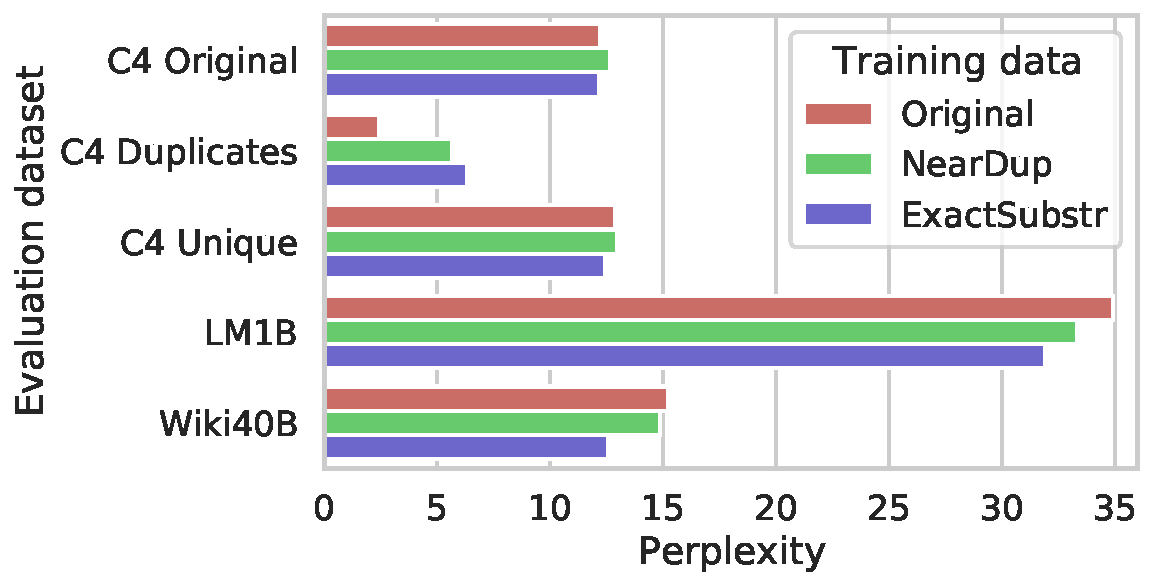
\includegraphics[width=0.6\linewidth]{figures/eval-xl-ppl_withLM1B.pdf}
    \caption{
Impact of deduplicating the training set on validation perplexity. In \textbf{(a)}, we plot the results from T5 base (110M parameters) across three training runs with different random initializations. The black bar represent the lowest perplexity to the highest perplexity, and the colored bar the median perplexity. 
    In \textbf{(b)}, we plot the results from T5 XL (1.5B parameters).
For C4, we evaluate on \textit{C4 Original}, the original validation set; \textit{C4 Unique}, a subset of the validation set identified by \Approx{} as having zero matches across C4; and \textit{C4 Duplicates}, a subset of the validation set identified by \Approx{} as having a match in the C4 train set.
}
\label{fig:eval-ppl}
\end{figure}

We computed the perplexity of our trained models on the validation sets of LM1B and Wiki-40B, and on subsets of the C4 validation set (Figure \ref{fig:eval-ppl}).
For the base size, we observe that all models have similar perplexity on the original C4 validation set and on validation set examples that were identified as unique (no near-duplicate in either train or validation).
However, both models trained on deduplicated data have significantly higher perplexity on validation set examples that have duplicates in the training set than the model trained on the original C4. \Exact-deduplicated results in higher perplexity than \Approx-deduplicated.
These trends holds true for the XL sized model as well.
While this may suggest \Exact{} duplication results in models least overfit on the train set, note that both of these techniques have
used separate duplicate thresholds and a different choice of thresholds could change the results.

When evaluating on the validation sets of LM1B and Wiki-40B, we found that models trained on \Approx-deduplicated C4 consistently achieved lowest perplexity.
\Exact{} deduplication decreases perplexity of the XL model by almost 3 points perplexity on Wiki-40B which is much larger than the variation of about 1 point perplexity we observed in the base models.
This is despite seeing fewer tokens of training data overall.

Lastly, we note all our XL models achieved  <35 perplexity on LM1B, which is less than the 42.16 perplexity reported for the 1.5B GPT-2 using a vocabulary the same size as ours.


\subsubsection{Impact on Generated Text}
\label{sec:memorization-results}
Data duplication has the effect of biasing the trained LM towards particular types of examples. 
This can contribute to a lower diversity of generations, and increased likelihood that the generated content is copied from the training data \citep{carlini2020extracting}.
For our generation experiments, we use top-$k$ random sampling with $k=50$ and experiment with prompted and unprompted generation.

\begin{table}[t]
    \centering
    \small
% \begin{tabular}{rrrrrr}
% \toprule
%  \multicolumn{2}{c}{Original Dataset} & \multicolumn{2}{c}{\Approx{} Deduplicated} & \multicolumn{2}{c}{\Exact{} Deduplicated} \\
%  \multicolumn{1}{r}{1} & \multicolumn{1}{r}{2} & \multicolumn{1}{r}{1} & \multicolumn{1}{r}{2} & \multicolumn{1}{r}{1} & \multicolumn{1}{r}{2} \\
%  \midrule
% 0.01372 & 0.01108 & 0.00122 & 0.00177 & 0.00082 & 0.00110 \\
% \bottomrule
% \end{tabular}
\begin{tabular}{l|rr}
\toprule
Model & 1 Epoch & 2 Epochs \\
\midrule
XL-\Original & 1.926\% & 1.571\% \\
XL-\Approx & 0.189\% & 0.264\% \\
XL-\Exact & 0.138\% & 0.168\% \\
\bottomrule
\end{tabular}
\caption{When generating 100k sequences with no prompting, over $1\%$ of the tokens emitted from a model trained on the original dataset are part of a 50-token long sequence copied directly from the training dataset. This drops to $0.1\%$ for the deduplicated datasets.}
\label{tab:memorizations_no_prompt}
\end{table}
We first evaluate memorization tendencies in the case where the model is asked to generate text without any prompt sequence.
We generate 100,000 samples, each up to 512 tokens in length.
For each generated token, we say the token is memorized if it is part of a 50-token substring that is exactly contained in the training data.
On XL-\Original, over 1\% of the generated tokens belong to memorized sub-sequences (see Table~\ref{tab:memorizations_no_prompt}).
This is $\sim10\times$ more memorization than XL-\Exact{} or XL-\Approx.
Some example subsequences that were copied verbatim from the train set can be found in Table \ref{tab:exact_substr_examples}.

% Table generated by Excel2LaTeX from sheet 'exact_example'
\begin{table*}[h]
  \centering
  \caption{A selection of substrings identified by \Exact{} as being in C4 multiple times. The number of times this exact substring occurs in C4 is also given.}
  \small
    \begin{tabular}{p{0.8\linewidth}|r}
    \toprule
    \multicolumn{1}{c|}{\textbf{Text}}  & \multicolumn{1}{c}{\textbf{Freq in C4}} \\
    \midrule
    HD wallpaper. This wallpaper was upload at April 19, 2019 upload by admin in.You can download it in your computer by clicking resolution image in Download by size:. Don't forget to rate and comment if you interest with this wallpaper. &            40,340  \\
    \hline
    to the address posted below. Include our failure information form,a packing slip with your Company name, contact person, and Email address or phone number. Upon receipt of your repair, we\textbackslash{}'ll inspect it and then contact you with a quote or evaluation notice. Normal turn aro\newline{}und for repair is 5 to 7 business days, with "Rush Repair" available. &              5,900  \\
    \hline
    is a great place to begin your search. Whether you are a first-time home buyer or you are already familiar with the home buying process, you can be assured that you have the best tools and the perfect agent available to help with your &              5,358  \\
    \hline
    pics at these awesome group starting P letter. Desktop wallpapers were first introduced way back in the 1980s and have gained immense popularity since then. It is possible to come across more than 80 million sites on the web offering some sort of wallpaper. &                 848  \\
    \hline
    flowers will let them know you're thinking of them and wishing them well. Cheerful yellow flowers bring their own sunshine and will get right to work on lifting spirits, and a colorful vase will bring loads of smiles to friends and visitors! Get Well flower arrangements from &                 479  \\
    \hline
    our premier 24 hour emergency* plumbing and heating solutions. We realise that when your heating fails or pipes and drains leak it can cause havoc with your routine and even cause damage to your property. When a plumbing problem occurs that requires an immediate response we provide qualified local plumbers throughout &                   56  \\
    \hline
     is to remove all images that violate copyrights. Please contact us to request that images be removed or to assign proper credit. The images displayed on this site may be used for Free or educational purposes only. If you would like to use any of the images displayed on this site for any other purpose, please obtain permission from the owner. www. &                   48  \\
     \hline
     list of fishing locations, providing interactive maps that show each location's GPS coordinates, nearby facilities (like restaurants, gas stations, marinas and fishing shops), their current and forecasted weather and, if available, their water conditions.\textbackslash{}nFind any of the 8 &                     5  \\
     \hline
    . Dyer, Ph.D., is an internationally renowned author and speaker in the field of self-development. He's the author of 30 books, has created many audio programs and videos, and has appeared on thousands of television and radio shows. &                     5  \\
    \bottomrule
    \end{tabular}%
  \label{tab:exact_substr_examples}%
\end{table*}%





% Table generated by Excel2LaTeX from sheet 'exact_example_in_generated'
\begin{table*}[h]
\caption{A selection of substrings generated by XL-\Original{} with no prompting (and top-$k$ with $k$=50) that were identified by \Exact{} as being in C4 multiple times. The number of times each substring was found in C4 is given. We observe that most memorized generations tend to be from advertisements.}
  \label{tab:approx_gen_noprompt_examples}%
  \centering
  \small
    \begin{tabular}{p{0.8\linewidth}|r}
    \toprule
    \multicolumn{1}{c|}{\textbf{Generated Text}}  & \multicolumn{1}{c}{\textbf{Freq in C4}} \\
    \midrule
    , you'll need to be knowledgeable to make the very best decisions. We will make sure you know what can be expected. We take the surprises from the picture by giving accurate and thorough information. You can start by talking about your task with our client service staff when\newline{} you dial 888-353-1299. We'll address all of your questions and arrange the initial meeting. We work closely with you through the whole project, and our team can show up promptly and prepared. & 5,497 \\
    \hline
    then Waterside Lodge are well equipped for the task. Our fully equipped family sized lodges offer a comfortable luxurious stay for a fantastic price, giving you beautiful views of the lakes and the surrounding countryside. Offering luxurious self-catering holidays in our fully featured Scandinavian holiday lodges. Perfectly located to explore the beaches, coastline. All of our lodges are sized for 6 people and are furnished to the highest standards to ensure you have a stay like no other. At Waterside Lodge the stay itself is only half of the package, Waterside lodge is situated closely to the Heritage Coast which makes our lodges the perfect stay for anyone wanting to get away and have a relaxing countryside break from the city. Whilst you stay with us be sure to take advantage of all the activities Waterside Lodge has to offer. Such as the use of our on-site fishing lakes for the keen fisherman, free internet access, outside relaxation areas, comfortable lounges and much more. & 571 \\
    \hline
    you are only looking to find rent to own homes in your city or are open to exploring all kinds of rent to own home listings, our database does it all. One of the best aspects of iRentToOwn.com is that, besides options to rent to buy a house, it has numerous other categories of home sale options. These include bank foreclosure homes, pre-foreclosure homes, short sales, HUD/government foreclosures, auction homes and owner-financing/FSBO (For Sale By Owner) homes. With help from the convenient search features offered by our site, shoppers are able to find their ideal lease to own home, real estate company, and more in South & 51 \\
    \hline
    , IL employs journeyman as licensed to work by themselves, without direct supervision, installing wiring, outlets and fixtures. Our journeyman also does service work, troubleshooting when a breaker fails or a light stops working. Our journeyman does not offer permits that must be issued by our master. Our journeyman follows our master's plans and directions. Our journeyman's responsibilities will vary based on the work that needs to be done. Our journeymen are skilled with residential, commercial and industrial installations and repairs.ust work from six years as an apprentice, under direct supervision of our master, and pass a journeyman test. This person also must have some classroom education on the National Electrical Code and fundamental electricity in a technical school a program affiliated with the National Joint Apprenticeship Training Council. Journeyman training combines hands-on work with education on basic electricity. & 6 \\
    \hline
    combustion process of a petrol engine is never perfect. Dangerous gases, such as nitrogen oxide, carbon monoxide and hydrocarbons will arise and it is the job of the catalytic converter to reduce these to safer emissions. These cat converters can fail by becoming clogged, or if the engine has bad exhaust valves or the plugs fail, causing unburned fuel to overheat the converter. Mettam's Mufflers can resolve these issues with your Karr & 5 \\
    \hline
    ,ANDREW Find the ancestral town: Many a researcher is stuck behind records that say, BIRTHPLACE: IRELAND without saying where in Ireland, or whatever other country. Remember that your immigrant ancestor's siblings probably were born in the same ancestral town, so check all o\newline{}f their records, too. Around 1900, the Roman Catholic churches reported marriages to the churches where the persons were baptised, and before the wedding, they would require a baptismal certificate from that church, without marriage notations, to make sure that the persons were no\newline{}t already married, ordained, or whatever, and were free to marry. Do check the Catholic records especially for ex loco and the home town. If your ancestor's sister had a daughter who generated a marriage or death record saying, MOTHER'S BIRTHPLACE: and the exact town, then y\newline{}ou know where to start searching for records that will confirm it is your ancestor's home town. BEWARE: Just because you find a family with the same names does not mean they are the same family, as they could very well be an unrelated family from a different town in the same an\newline{}cestral country. The webmaster has learned this. One clue was that one family was still having babies in Potenza city, Italy while the other was having babies in Colorado, U.S.A. & 2 \\
    \hline
    will not want to search for Power Washing companies in Wyoming on an extensive basis. The service personnel will be at your doorsteps through online or phone booking. The power wash solutions offered by us are matchless and you can compare with others in Winfield, IL. The power wash services offered by us are very economical. Gutter brightener will be applied which will be followed by cleaning through double scrub. The cleaning will be done by using a soft bristle brush. The bond and contaminants will be released in an effortless manner. & 1 \\
    \hline
    Z3 Plus are valid in all major cities of India like Delhi, Gurgaon, Noida, Mumbai, Chennai, Bangalore, Hyderabad, Kolkata, Pune, Ahmedabad, Coimbatore, Lucknow, Trichy, Madurai, Trivandrum, Mysore, Jaipur, Chandigarh, Pondicherry, Bhopal, Patna, Bhubaneswar, Amritsar, Cochin, \newline{}Allahabad, Srinagar, New Delhi, Surat, Ludhiana, Navi Mumbai, Ghaziabad, Bengaluru, Indore, Nagpur, Thane, Agra, Meerut, Ranchi. The delivery feasibility and charges may be varying, hence for them please check with the particular seller or store. & 1 \\
    \bottomrule
    \end{tabular}%
\end{table*}%


\begin{figure}
    \centering
    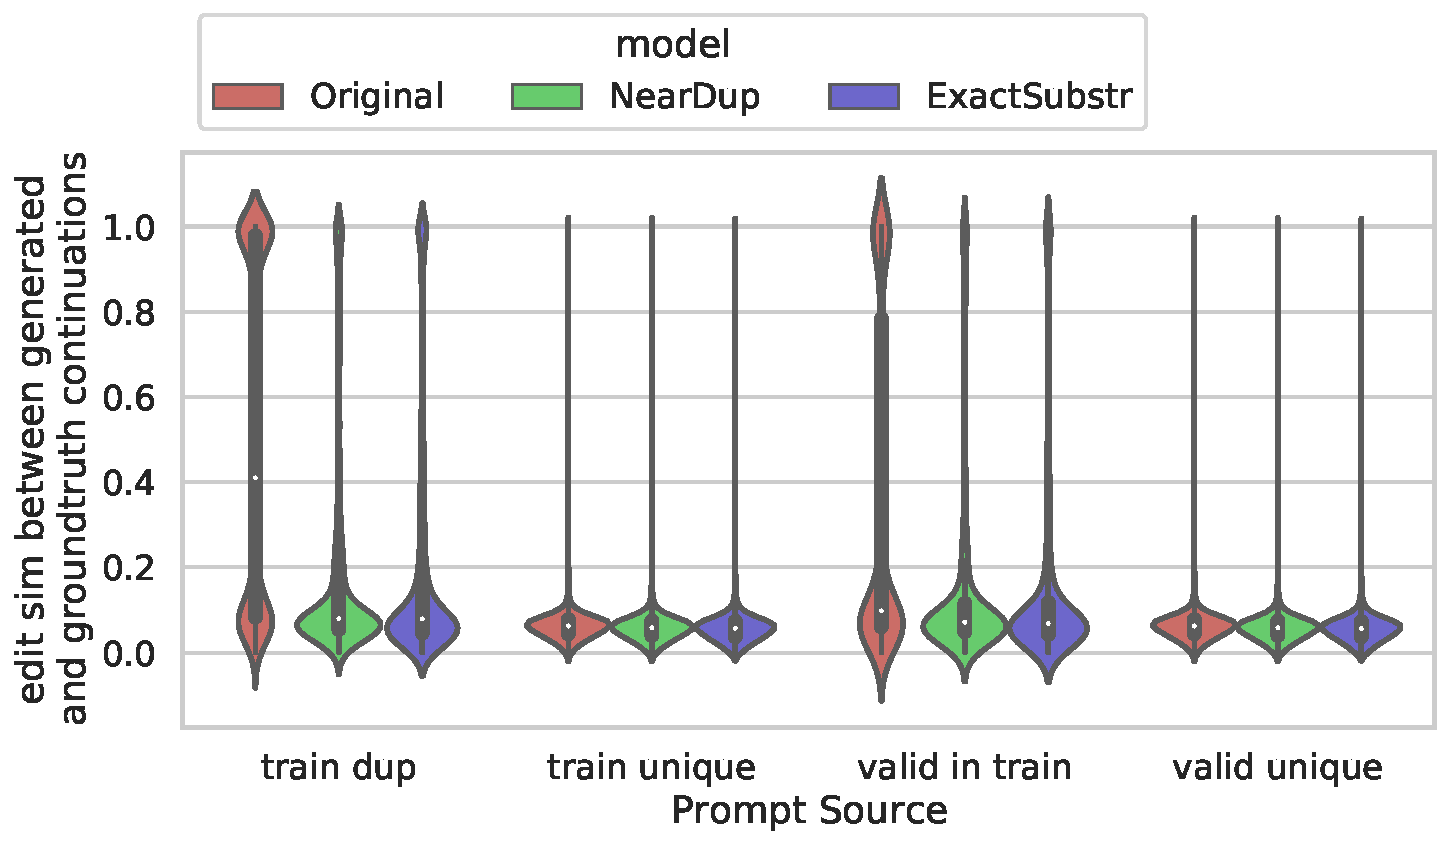
\includegraphics[width=\linewidth]{figures/memorized_continuations_distribution.pdf}
    \caption{Memorized continuations distribution}
    \label{fig:mem-cont-dist}
\end{figure}

\begin{figure}
    \centering
    \small
    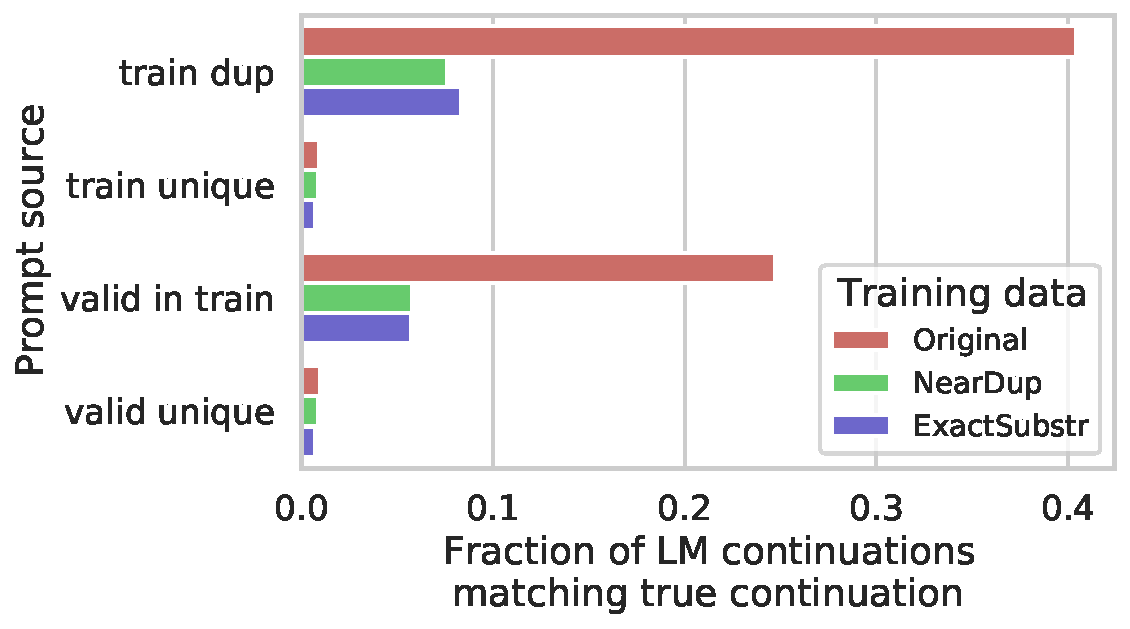
\includegraphics[width=0.6\linewidth]{figures/memorized_continuations_fraction}
    \caption{The proportion of generations which have edit similarity above 0.8 with the groundtruth continuation when using the LM to generate continuations for 32-token prompts identified by \Approx{} as either duplicated or unique.}
    \label{fig:ground-truth-continuation}
\end{figure}

In most real use cases, language model generation is controlled by providing a prompt for the model to continue.
We experiment with four possible prompt sources: training examples identified by \Exact{} as having near-duplicates in the train set (train dup), training examples identified as unique (train unique), validation set examples with a near-duplicate in the train set (valid in train), and validation set examples identified as unique across all splits (valid unique).
We select the first 32 tokens of each example as the prompt, which means we can evaluate the fraction of generations which are near-duplicates with the ground-truth continuation for the prompt.
Figure \ref{fig:ground-truth-continuation} shows the proportion of generations which meet this requirement, while Figure \ref{fig:mem-cont-dist} shows the distribution in edit similarities between the generations and ground-truth continuations.
When the prompt comes from duplicate examples in the train set, XL-\Original{} reproduces the groundtruth continuation over 40\% of the time.
XL-\Exact{} and XL-\Approx{} still copy the groundtruth more often when the prompt comes from a duplicate example than when the prompt comes from a unique example, suggesting that more stringent deduplication may be necessary to remove memorization tendencies entirely. 

% \begin{table*}[]
%     \centering
%     \small
%     \begin{tabular}{ll|rr|rr|rr}
%     \toprule
%      &  & \multicolumn{2}{c}{Original eval set} & \multicolumn{2}{c}{Eval examples in train} & \multicolumn{2}{c}{ Unique eval examples} \\
%     Dataset & Model & \multicolumn{1}{c}{Count} & \multicolumn{1}{c}{Ppl} & \multicolumn{1}{c}{Count} & \multicolumn{1}{c}{Ppl} & \multicolumn{1}{c}{Count} & \multicolumn{1}{c}{Ppl} \\
%     \midrule
%     LM1B & Transformer-XL \citep{dai2019transformer} & 306,688 & 21.77  & 15,126  & 10.11  & & \\
%     % RealNews & GROVER-Base &  &  15.440 & & 13.771 \\
%     RealNews & GROVER-Base \citep{zellers2019defending} & 1,639,104 &  15.44 & 235,235 & 13.77 &  & 15.73  \\
%     RealNews & Grover-XL \citep{zellers2019defending} & &  &  & 7.68 & & 9.45 \\
%     \bottomrule
%     \end{tabular}
%     \caption{The perplexity of a trained language model on the official validation set and the perplexity on the valid set examples which were identified as near-duplicates of training set examples. \todo{finish up computing values}}
%     \label{tab:ppl_sota_models}
% \end{table*}


\begin{table}[]
    \centering
    \small
    \begin{tabular}{ll|rrr}
    \toprule
    Model & Dataset & \multicolumn{1}{c}{Orig} & \multicolumn{1}{c}{Dups} & \multicolumn{1}{c}{Unique} \\
    \midrule
    Transformer-XL & LM1B & 21.77 & 10.11  & 23.58  \\
    % RealNews & GROVER-Base &  &  15.440 & & 13.771 \\
    GROVER-Base  & RealNews & 15.44 & 13.77 & 15.73  \\
    GROVER-XL & RealNews & 9.15 & 7.68 & 9.45 \\
    \bottomrule
    \end{tabular}
    \caption{For each model, the perplexity of the official validation set (\textit{Orig}), valid set examples which were identified by \Approx{} as matches of train set examples (\textit{Dups}), and valid set examples identified by \Approx{} as unique (\textit{Unique}).
    Due to the size of the RealNews validation set, we evaluated on only the first 25k examples meeting each condition.}
    \label{tab:ppl_sota_models}
\end{table}

\subsubsection{Impact on Existing Models} \label{sec:eval-existing-models}
Train-test leakage does not just impact models trained on C4.
Table \ref{tab:ppl_sota_models} shows that
% the presence of a near-duplicate
the presence of near-duplicates of the evaluation set
% whether or not an evaluation example has a near-duplicate
in the train set has a significant impact on model perplexity for two standard models: Transformer-XL \citep{dai2019transformer}, which was trained on LM1B, and GROVER \citep{zellers2019defending}, which was trained on RealNews.
For Transformer XL, the perplexity halves on examples identified as near-duplicates.
For GROVER, the difference, though not quite as stark, is present in both model sizes considered.

Existing models also suffer from the problem of generating text from their train sets.
We find that $1.38\%$ of the tokens in the official release of 25k GROVER-Mega outputs
%\footnote{\url{gs://grover-models/generation_examples/generator=mega~dataset=p0.90.jsonl}}  % TODO SPACE
are part of verbatim matches in RealNews of at least length $50$.
Likewise, more than 5\% of the tokens in \textasciitilde 200k sequences outputted by GPT-Neo 1.3B \citep{gpt-neo} are part of a $50$ token matches of its training data, the Pile \citep{pile}.

\subsection{Discussion}
The focus of this paper is on the datasets used to train language models.
While recent work focused on documenting the potential harms that could arise from problematic datasets  \cite{bender2018data, gebru2020datasheets}, less work has been done to 
quantitatively analyze properties of real language modelling datasets, like \citet{dodge2021documenting} has done for C4.
Our paper provides analysis on one particular axis, that of data duplication.

Our experiments measured what could be quantified: the amount of duplicate content in common datasets, the effect of deduplication on trained model perplexity, and the reduction of memorized content in trained models through deduplication.
We do not focus on the nature of the data being removed by deduplication or memorized by LMs.

Privacy is an important subject for future work, as memorized training data has significant privacy consequences.
By this, we mean the standard privacy definition that a model should not reveal anything particular to the specific dataset it was trained on, as opposed to another training dataset from a similar distribution \citep{shokri2017membership}.\footnote{%
Another interpretation of privacy focuses on the sensitivity of the data involved, when a model is trained on and able to reproduce personal identifiers or other forms of ``private data.'' Our definition is more expansive.}
Training on standard datasets that have not yet been deduplicated results in models that are particularly sensitive to examples that happened to be repeated multiple times, and this has negative privacy implications.
For instance, it could violate a person's expectations of privacy if their publicly available personal data appeared in a different, surprising context.
Downstream applications of LMs, such as the game AI Dungeon\footnote{\url{https://play.aidungeon.io/}}, should also not output memorized content like adverts for real products. 

We stress that in our experiments, we do not distinguish between undesired memorized text (such as phone numbers), innocuous memorized text (common phrases), and text we may want to be memorized (such as a quote by a public figure), and instead treat all instances of the LM generating text that closely matches the training set as problematic.
While we qualitatively observed that much of the identified memorized content was relatively innocuous, a more systematic study of the risks associated with the detected memorization was beyond the scope of this work.

We also do not investigate the negative consequences of deduplication.
Some language tasks explicitly require memorization, like document retrieval or closed-book question answering. 
Also, text that gives attribution is often duplicated across documents, so
removing duplicate substrings could correspond to removing \emph{just} the attribution, which could result in models that learn the content without its attached attribution.
Deduplication is also not sufficient to remove privacy-sensitive data like bank passwords and medical records which should never be used in training data.

Ultimately, whether memorization is a desired property of a language model, or else risky and unwanted, depends
% both % TODO add back in
on the nature of the text that has been memorized and on the downstream applications of the trained model.
However, since the trend has been towards creating datasets and models that are application-agnostic, we encourage researchers to think carefully about the limitations of the data
% they have % TODO add back in
collected and the how the model's intended usage constrains what should be part of the training set. 
% For example, if the goal of training a language model is to be able to exactly reproduce text found on the internet, then perhaps deduplication does not make sense.
% However, for the vast majority of related work, the goal is to model human communication through language, which means training on low-quality highly duplicated text undesirable.
Developing techniques to memorize or forget specific sequences depending on the end application is a promising research direction. 

We encourage future language model research to perform dataset deduplication, either by training on the deduplicated datasets we release, using the deduplication tools we release, or following our approach to deduplicate datasets with new tools.

The exact technique used to perform deduplication is less important than performing stringent deduplication in the first place.
On the whole, deduplication does not harm, and sometimes improves, model perplexity, despite the fact that the deduplicated datasets are smaller and faster to train on.
It is especially important that there are no duplicates between the training and testing sets, because overlap here explicitly encourages selecting models that memorize the training data.
Lastly, deduplication helps to reduce some of the privacy concerns around LMs memorizing their training data.
